
\begin{subsection}{Overview}

We now turn to a discussion of the methods whereby we can compare our newly
developed anisotropic force field methodology to various
sum-of-spheres models. 
As is standard in ab initio force field development, we use a
straightforward metric to evaluate force field quality:
the accuracy with which a given force field functional form can reproduce
high-quality ab initio benchmark energies. Furthermore, and because the
functional forms introduced in \cref{sec:theory} directly affect only the
pairwise-additive portion of the intermolecular potential, we
concentrate our efforts on assessing force field with respect to benchmark
calculations of dimer interaction energies, which directly measure the
two-body portion of a system's total intermolecular interaction energy.
(When required, and as discussed in \cref{sec:co2}, many-body effects can be accounted for separately
and systematically using known methods).\cite{Yu2012b,McDaniel2014}
%
In addition to this primary metric for force field quality, we also evaluate our force
fields for their ability to reproduce select experimental properties.
Importantly, however, 
experimental predictions from an ab initio force field significantly depend, not only on the
fit quality of the pair potential, but also on the 
choice of benchmark electronic structure theory, treatment of many-body and/or quantum
effects, etc. 
Because these factors complicate comparisons to experiment, here
we treat experimental accuracy as an important, but secondary, metric for evaluating force
field accuracy. 

So as to systematically evaluate the effects of anisotropy on the development of
intermolecular potentials, we compare three types of models.
The first model, which we call \isoff, uses a completely isotropic description
of all energy components. Our second model, \isaff, accounts for long-range electrostatic
anisotropy by including multipolar contributions (up to
quadrupoles), but uses an isotropic model for all other terms in the
intermolecular force field.
Note that this model is virtually identical to the \isaffold
model developed in \cref{ch:isaff}, and that this manner of partially
treating anisotropy is very similar in spirit to the popular AMOEBA\cite{Ren2003,Shi2013}
methodology. Finally, we develop \anisoff, which selectively incorporates anisotropy into all
energy components (aside from long-range polarization) of the intermolecular potential.
This model, which we also refer to with the moniker \mastiff (a
\textbf{M}ultipolar, \textbf{A}nisotropic, \textbf{S}later-\textbf{T}ype
\textbf{I}ntermolecular \textbf{F}orce \textbf{F}ield), treats all
electrostatic interactions via a multipole expansion with up to quadrupolar
contributions, and includes anisotropic parameters for other terms of the force field
(short-range interactions plus dispersion) for heteroatoms, atoms in
multiple bonding environments, and associated hydrogens. A complete list of anisotropic atom types is
given in the \cref{sec:mastiff-local_axis_defs}.

\end{subsection}
\begin{subsection}{Accuracy: Comparison with DFT-SAPT}

For each of the 91 dimer combinations described in \cref{sec:methods},
parameters were fit to reproduce \sapt energies calculated for 1000 different
relative orientations of the constituent monomers. 
From these `dimer-specific' fits, and as in
described in \cref{ch:isaff},\cite{VanVleet2016} we then averaged the
root-mean-squared (\rmse) and mean signed errors (\mse) from each of the 91
fits to produce so-called `characteristic \rmse/\mse', metrics
representative of the errors associated with a given force field methodology.
Typically, because the absolute magnitudes of the various energy components
become large in the repulsive portion of the potential, these characteristic
errors are dominated by repulsive
configurations. As such,
we have also calculated `attractive
\rmse/\mse' (a\rmse/a\mse), defined as the characteristic errors for the subset
of configurations with net attractive total interaction energies. 
All computed characteristic \rmse are shown in \cref{fig:rmse}.
Unless otherwise stated, results in this section refer
exclusively to the `Dimer-specific' fits in \cref{fig:rmse}, with an
explanation and full discussion of so-called `Transferable' fits given in
\cref{sec:transferability}.

    %%%%%%%%%%%% Average RMSE %%%%%%%%%%%%%%%
    \begin{figure}
    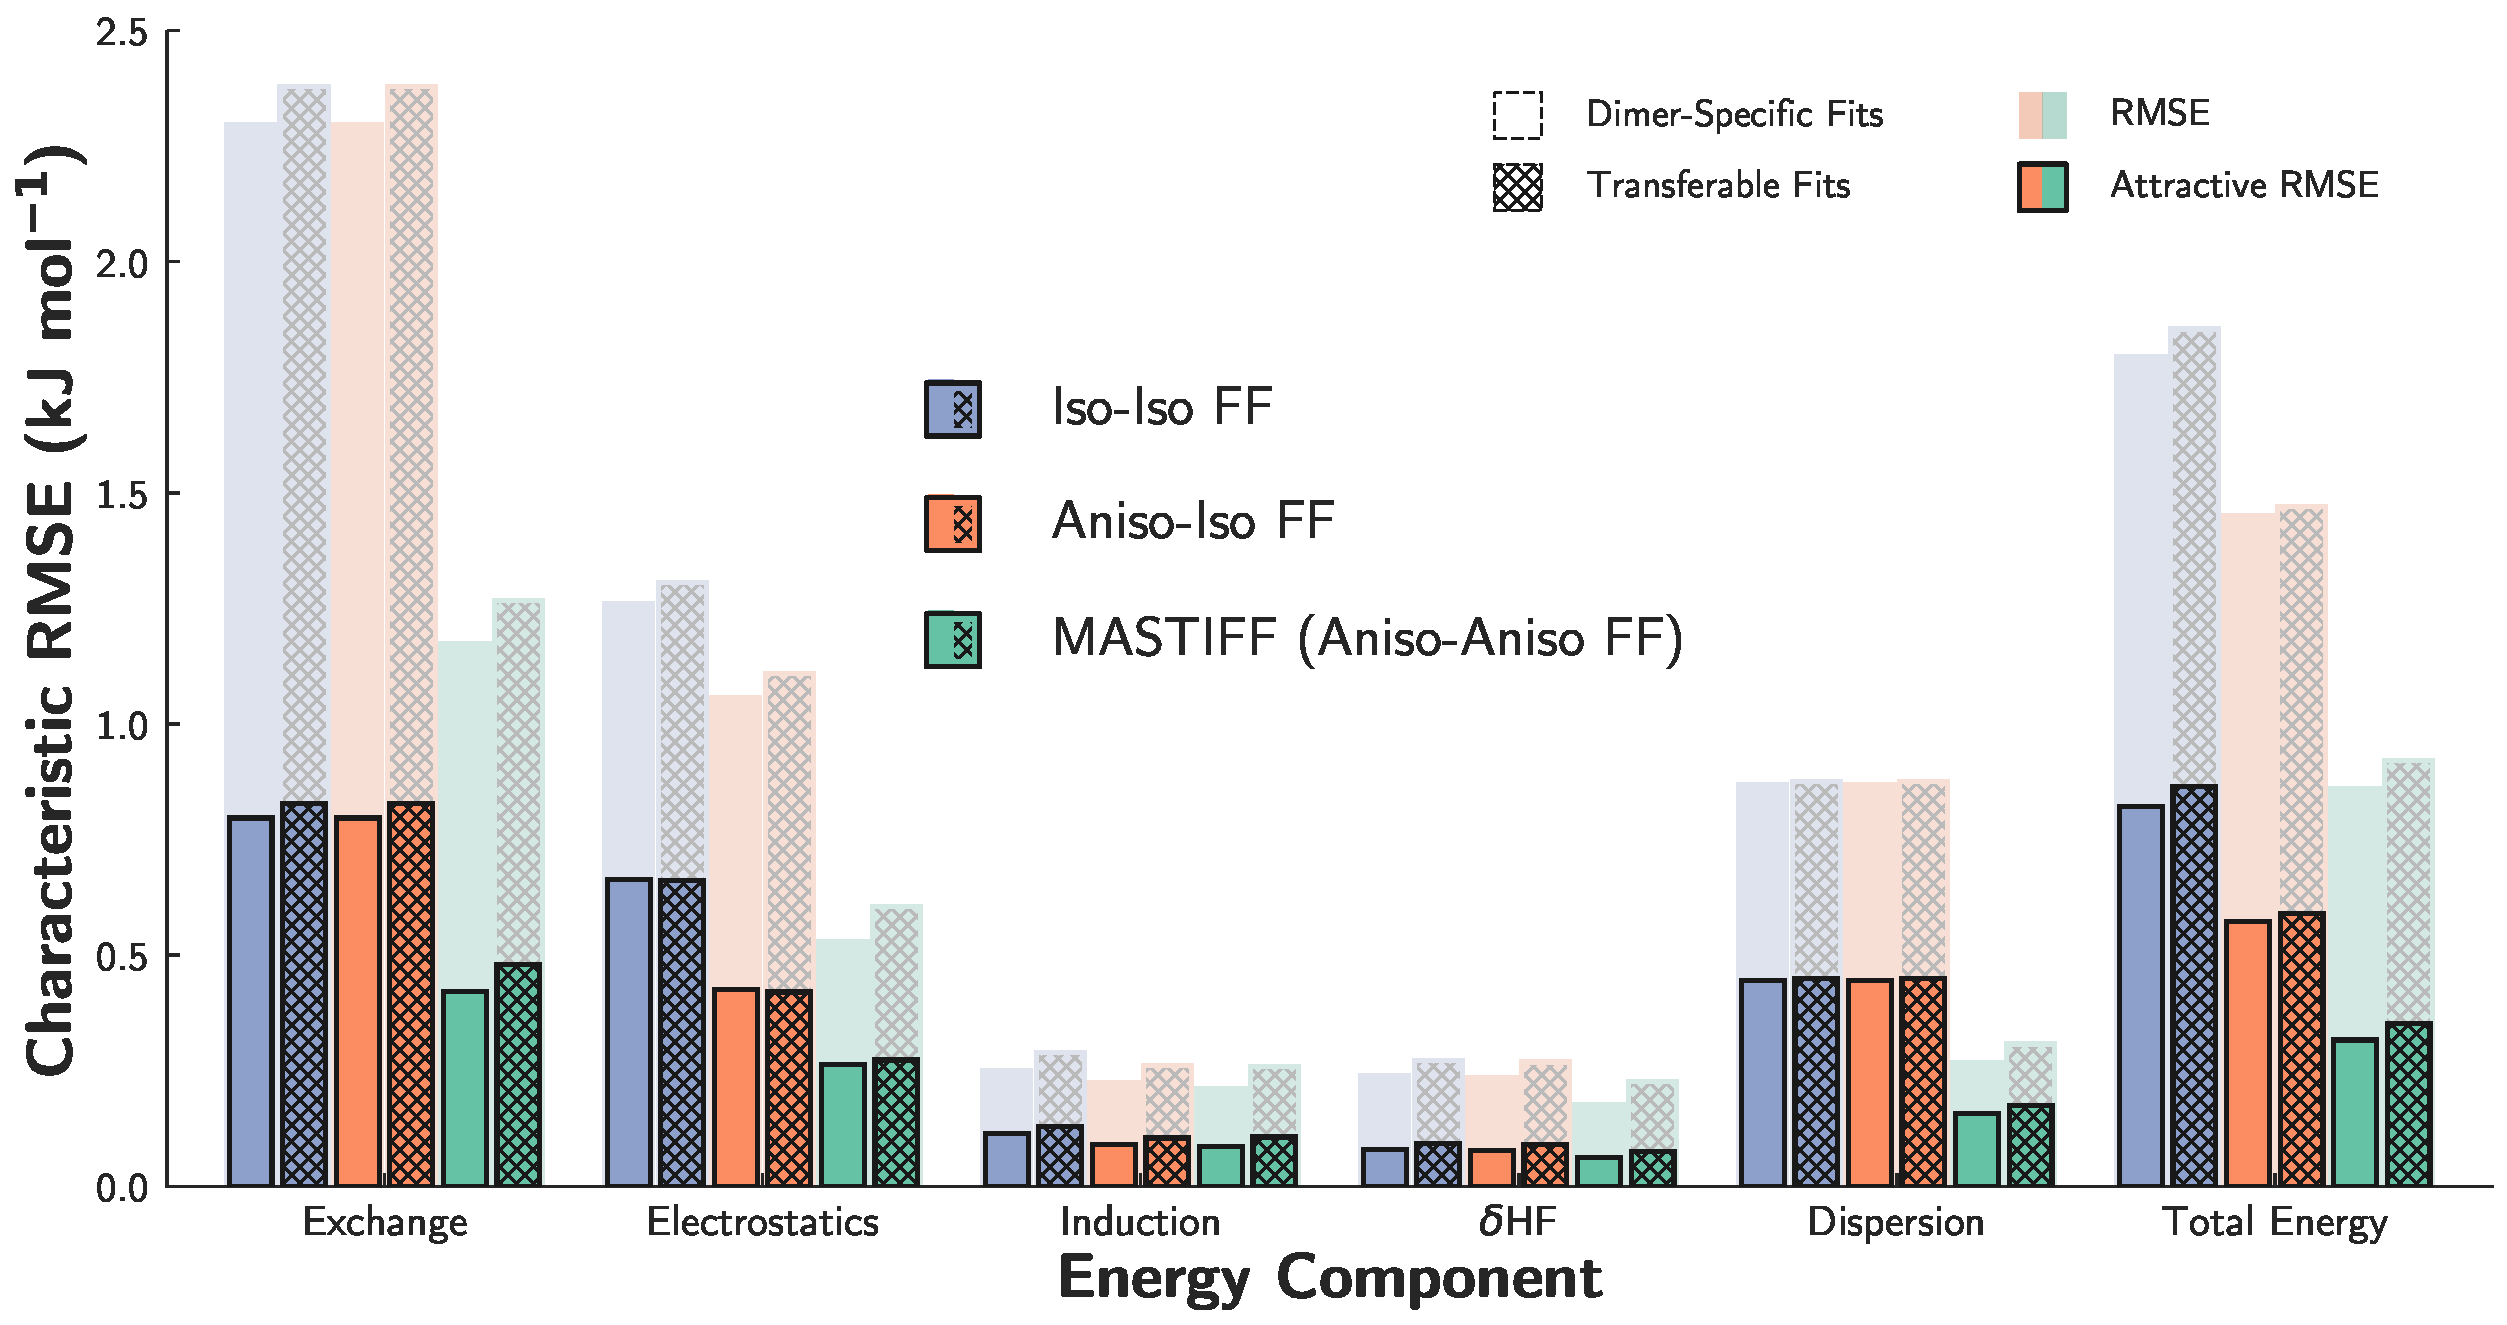
\includegraphics[width=0.9\textwidth]{anisotropic/rmse_comparisons/transferability_rmse_errors.pdf}
    \caption{
    Characteristic RMSE (as described in the main text) for the \isoff
(purple), \isaff (orange), and \mastiff (green) over the 91
    dimer test set. The semi-transparent bars represent total RMSE
    for each energy component, while the smaller solid bars represent `Attractive'
    RMSE, in which repulsive points have been excluded. For each force field,
    two types of fits, dimer-specific (solid) and transferable (hashed lines),
    are displayed; see \cref{sec:transferability} for details. Finally, note that, for \isoff and \isaff, only the electrostatic
    and total energy \rmse's differ. 
            }
    \label{fig:rmse}
    \end{figure}
    %%%%%%%%%%%% Average RMSE %%%%%%%%%%%%%%%

Based on the characteristic \rmse shown in \cref{fig:rmse}, both \isaff
and \mastiff offer substantial improvements over the completely isotropic model
\isoff. Though unsurprising, given the well-studied importance of higher-order
electrostatic multipole moments, \isaff shows reduced \rmse/a\rmse that are (depending on the exact
error metric used)
roughly 30\% smaller than \isoff. 
Both \rmse and a\rmse measures showing similar gains in accuracy,
indicating that inclusion of higher-order multipoles (henceforth
`multipolar electrostatic anisotropy') is important in both
attractive and repulsive regions of the potential. Crucially, inclusion of
additional `short-range anisotropies' (anisotropic
interactions arising from overlap of monomer electron densities, namely
exchange-repulsion and electrostatic/inductive charge penetration) and
long-range `dispersion anisotropy' yields a \emph{further} 40\% reduction in
\rmse/a\rmse for \mastiff as compared to the \isaff.
This latter
result is highly important, as it suggests that, for the generation of highly
accurate ab initio potentials, the combination of short-range
and dispersion anisotropies 
are just as important to include as
multipolar electrostatic anisotropy. Indeed, this substantial increase in
force field accuracy, which arises from a full treatment of anisotropic
effects, and is independent of improvements from multipolar electrostatic anisotropy, 
is one of the most important findings in the present Chapter.
In summary, and encouragingly, the combination of multipolar electrostatic, short-range, and
dispersion anisotropies result in an overall 60\% reduction in \rmse/a\rmse when
comparing \isoff to \mastiff. 

To see exactly how an inclusion of anisotropy impacts each component of the
potential, \cref{fig:rmse} also displays characteristic \rmse/a\rmse for each term
in the force field description as compared to DFT-SAPT. Immediately, one can
see that (aside from induction, discussed below),
an inclusion of atomic-level anisotropy greatly improves the description of
each energy component. Unless otherwise stated, here we report results
for a\rmse and
dimer-specific fits, though similar values are obtained for overall \rmse and
for transferable fits.
Compared to \isoff, exchange errors in \mastiff
are reduced by 47\%. Electrostatic errors are reduced by an even larger
60\%. By evaluating the ratio of electrostatic errors between different
models, we find that $\sfrac{\text{a\rmse \isaff}}{\text{a\rmse \isoff}} = 0.64$
and $\sfrac{\text{a\rmse \mastiff}}{\text{a\rmse \isaff}} = 0.62$, suggesting
that \emph{both} higher-order multipoles and anisotropic charge penetration
terms are necessarily to obtain an accurate description of the DFT-SAPT
electrostatic energy. Finally, via an inclusion of dispersion anisotropy,
a\rmse for dispersion are reduced by a significant
65\%. 
%% Especially for dispersion, some of this error reduction may simply be due to
%% the increased number of free parameters associated with anisotropic atom types.
%% (For dispersion, no free parameters are fit for isotropic atom types, while up
%% to three parameters are fit for anisotropic atom types. For 
%% functional forms describing penetration, by contrast, one free parameter is
%% fit for isotropic atom types, while up to four free parameters are fit for
%% anisotropic interactions). If we relax the constraint from
%% \cref{eq:ff_details} that $\Adisp{} = 1$, thus fitting at least one free
%% parameter per isotropic atom type, we find a somewhat smaller improvement factor for
%% dispersion a\rmse of 47\%, which is more similar to what was observed for the
%% exchange energy. Regardless, it is qualitatively clear that dispersion
%% anisotropy plays an imporant role in determining overall force field accuracy.

Though the trends for exchange, electrostatics, and dispersion universally
suggest the importance of including atomic-level anisotropy, trends for terms
describing the physics of polarization and charge-transfer (represented in
DFT-SAPT by induction and
\dhf) are less encouraging. On the one hand, including higher-order multipoles
substantially lowers \rmse for induction, with $\sfrac{\text{\rmse \isaff}}{\text{\rmse \isoff}} = 0.70$. 
Because both \isoff and \isaff use isotropic polarizabilities, and because the
induction energy fundamentally depends only on the polarizabilities and the
static electric field, this
result is clearly due to an improved treatment of the static electric field
via anisotropy of the multipolar electrostatics.
Once again, this
suggests that an 
anisotropic treatment of long-range electrostatics is crucial for accurate
force field development. On the other hand, our functional form for anisotropic short-range
induction (\cref{eq:ff_form} and \cref{eq:v_aniso}) leads to no improvement in the
induction \rmse, with $\sfrac{\text{\rmse \isaff}}{\text{\rmse \isoff}} =
0.97$. This observed lack of improvement is likely due to a combination of
factors. First, and perhaps most importantly,
we have chosen in this Chapter to use isotropically-averaged dipole
polarizabilities, but as with
electrostatics, anisotropy and higher-order terms have been shown to be important in in the multipole
expansion of atomic dipole polarizabilities. 
\cite{Stone2007,Misquitta2007a,Misquitta2008b,Misquitta2016,Harder2006}
Second, and though probably a smaller source of error,
it is also unclear how to optimally
model the distance dependence of the induction energy at short
intermolecular separations, where penetration and charge-transfer effects
become important and the long-range polarization terms must be damped. 
\cite{VanVleet2016,Liu2017,Misquitta2013,Thole1981} 
Given that the more elaborate short-range form of the 
\mastiff induction model does not result in a tangible improvement, it is quite possible
that alternative formulations are required for an accurate treatment of highly
anisotropic induction.

    %% %%%%%%%%%%%% H2O Comparison %%%%%%%%%%%%%
    %% \begin{figure}[ht]
    %% 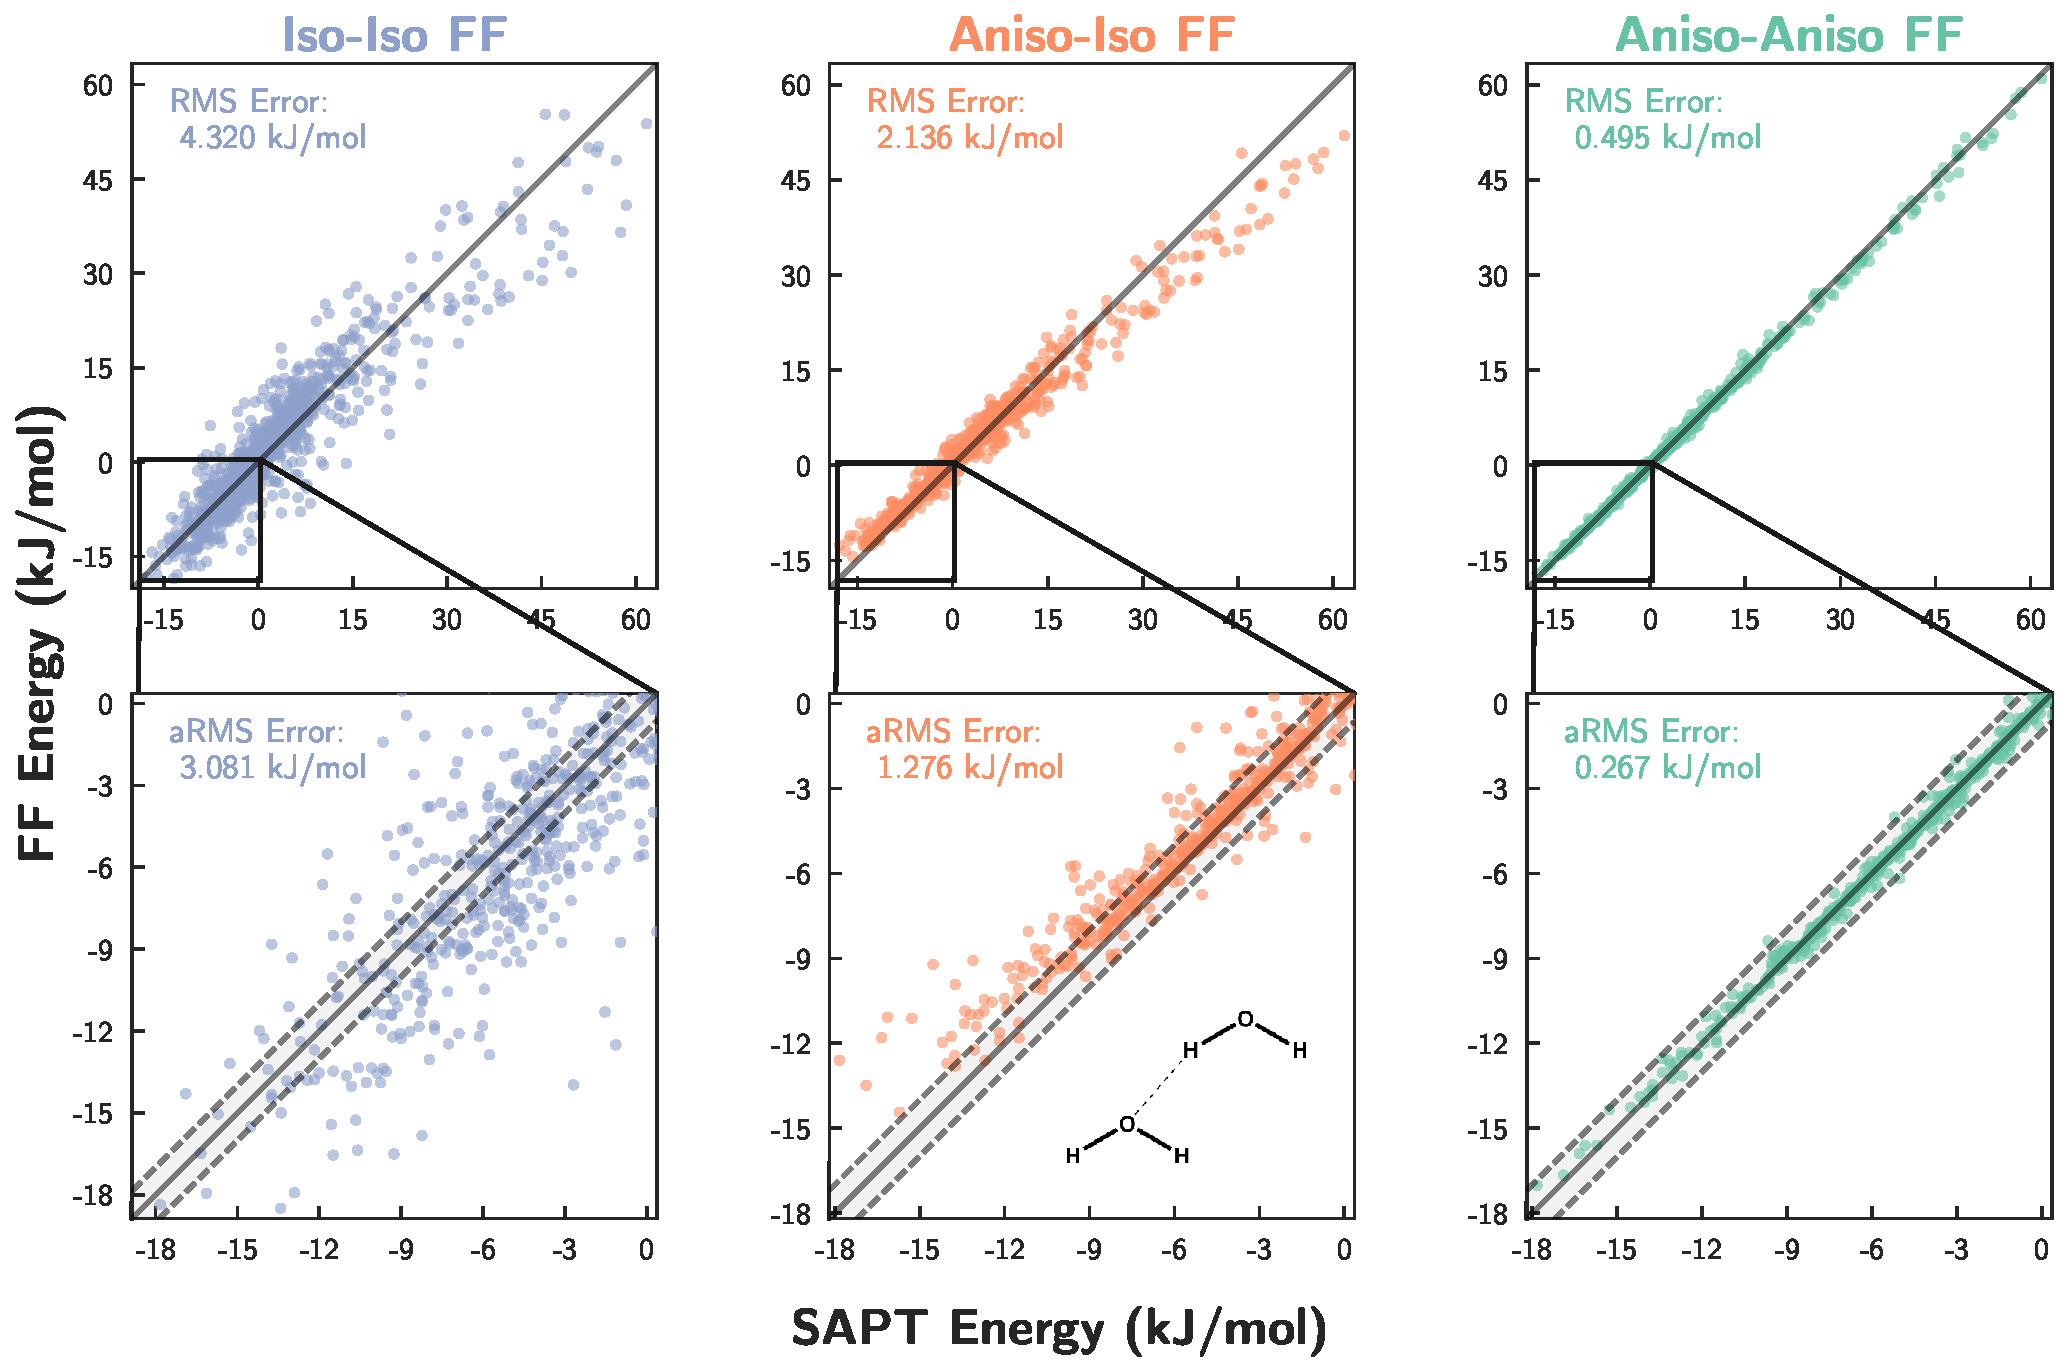
\includegraphics[width=0.9\textwidth]{figures/h2o_h2o_comparison.pdf}
    %% \caption{
    %%     Force field fits for the water dimer using \isoff (purple), \isaff (orange,
    %%     and \mastiff (green).
    %%     Fits for the total energy are displayed along
    %%     with an inset of the attractive regions. The solid $y=x$ line 
    %%     indicates perfect agreement between reference energies and each force field,
    %%     while dotted lines represent $\pm1$ \kjmolold error bounds. \rmse and a\rmse as in
    %%     the main text.
    %%         }
    %% \label{fig:h2o}
    %% \end{figure}
    %% %%%%%%%%%%%% H2O Comparison %%%%%%%%%%%%%

To further analyze the effects of anisotropy on a molecule-by-molecule basis, we have calculated
`improvement ratios', defined as 
$\sfrac{\text{a\rmse \isoff}}{\text{a\rmse \mastiff}}$,
for each energy component and for
each homomonomeric species in the test set, results for which are shown in
\cref{tab:ratios}. 
(Improvement ratios for heteromnomeric species are given in the \si of
\citen{VanVleet2017}, and we additionally provide
scatter plots of each homomonomeric force field fit in \cref{sec:mastiff-fits}.)

The most striking observation from the data presented in \cref{tab:ratios} is that
the improvement ratios vary considerably with molecule. For example, with water
the a\rmse is improved by an order of magnitude when anisotropy is included. On
the other hand, no improvement is seen for hydrocarbons such as ethane and
methane (also see the \cref{sec:mastiff-fits}). Consequently, anisotropy in the short-range expansions
may be necessary for only some atoms types (see \cref{sec:conclusions}). For the molecules
studied in our test set, and in line with chemical intuition, we have found
anisotropy to be particularly important for 
heteroatoms, $\pi$-bonded atoms,
and all hydrogens bonded to anisotropic heavy atoms. 
Appealingly, this distinction between anisotropic and
isotropic atom types 
simplifies force field parameterization and can enable more efficient molecular
simulation (via a more cost-effective treatment of multipolar electrostatics) without sacrificing force field accuracy.
Note that the current empirically-determined
definitions of anisotropic atom types
match both chemical intuition and the more quantitative measures
of atomic anisotropy proposed by other groups.\cite{Kramer2014,Wheatley2012}


    %%%%%%%%%%%% Error Ratios %%%%%%%%%%%%%%%
    \begin{table}[ht]
    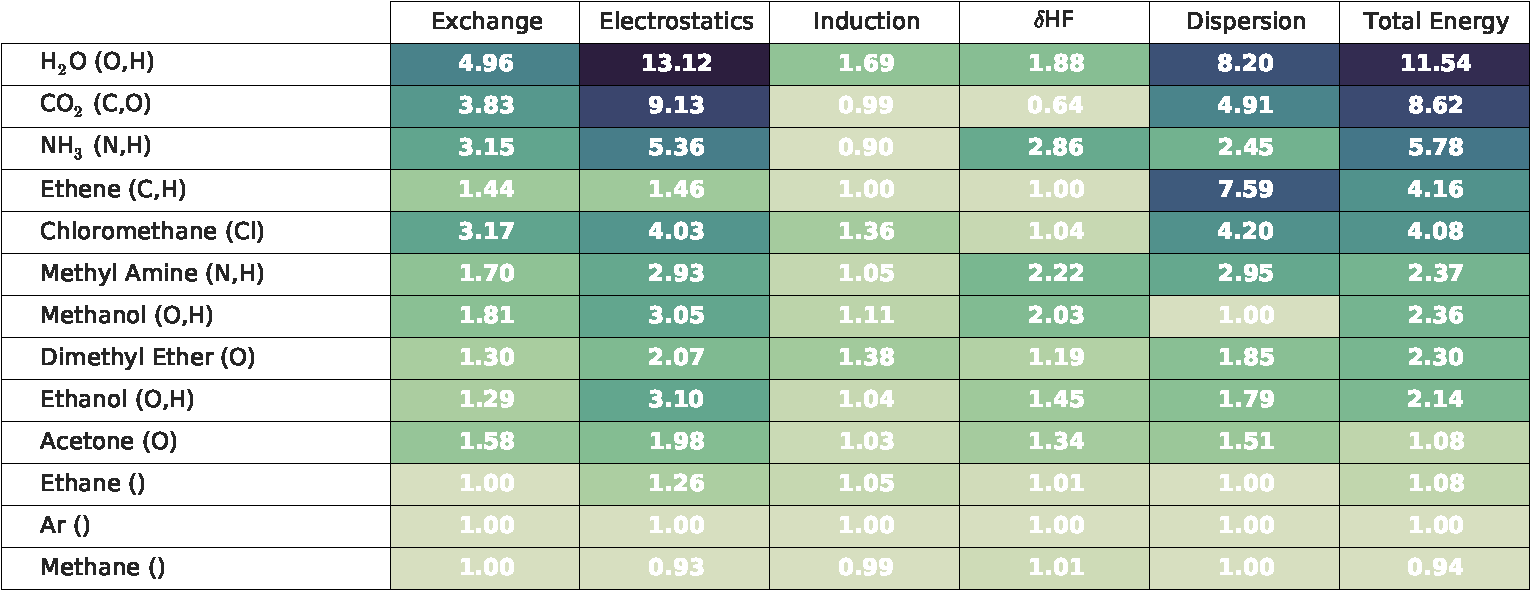
\includegraphics[width=0.9\textwidth]{anisotropic/figures/homodimer_error_ratios.pdf}
    \caption{
`Improvement Ratios' for each homomonomeric species in the
91 dimer test set. For each dimer and energy component, the improvement ratio
is calculated as the ratio of a\rmse between \isoff and \mastiff; values
greater than 1 indicate decreased errors in the anisotropic model. Entries have
been ordered according to the improvement ratio for the total energy.
            }
    \label{tab:ratios}
    \end{table}
    %%%%%%%%%%%% Error Ratios %%%%%%%%%%%%%%%


In general, the ordering of improvement ratios for exchange,
electrostatics, dispersion, and the total energies are reasonably correlated. (As stated above, our model
for anisotropic induction interactions is rather poor, and hence the
improvement ratios for induction and \dhf are relatively uncorrelated with the
other components. A good model for anisotropic induction and
\dhf might easily change this result). Physically speaking, all atomically-anisotropic
interactions arise from the same source (atomically-anisotropic
electron densities), and so the observed correlation might have been expected.
Nevertheless, there are some exceptions to this trend, such as with ethene and
acetone.
For ethene, relatively modest improvement ratios (roughly 1.4) are seen for exchange and
electrostatics, whereas dispersion shows a much greater improvement ratio of
7.6. Since ethene homomonomeric interactions are dispersion-dominated, the
improvement ratio for the total energy then roughly corresponds to that of dispersion.
A larger test set (particularly one which includes more non-polar
aromatic species) would be necessary to assess the generality of this result.
For acetone, there is good correlation between the improvement ratios for
exchange, electrostatics, and dispersion, which might lead one to suspect that
the total energy improvement ratio would also be around 1.5-2.0. Nevertheless, for this molecule, the
isotropic model benefits from error cancellation between energy components,
and the total energy a\rmse between isotropic and anisotropic models are
rather similar. 

Crucially, 
electrostatics is most definitely not the only intermolecular interaction for which
atomic-level anisotropy improves model quality. Indeed, for molecules like ethene, multipolar
anisotropy in the electrostatic model is relatively unimportant, whereas dispersion anisotropy is
essential for accurately modeling the $\pi$ interactions.
Thus, for a given system, multipolar electrostatic, dispersion, and/or short-range
anisotropies may all be important, and all relevant 
anisotropies must be accounted for in order to obtain good intermolecular
models.

\end{subsection}
\begin{subsection}{Transferability: Comparison to DFT-SAPT}
\label{sec:transferability}

From the above results it is clear that, when explicitly parameterized, an
inclusion of anisotropy can greatly enhance the accuracy of an intermolecular
potential. Nevertheless, for standard force field development, force field
parameters must be \emph{transferable} in order to be
useful in the accurate prediction of intermolecular
interactions in new chemical and/or physical environments. Indeed, in comparing
simpler models to ones that
introduce additional complexity, 
there is an ever-present danger that any accuracy
gains from the more complex functional form are simply due to
over-fitting or error cancellation,\cite{Hawkins2004} ultimately resulting in an overly-complex
model with poor predictive ability and limited transferability. 

We have previously shown how, with models
similar to \isoff\cite{McDaniel2013,Schmidt2015} or
\isaff,\cite{VanVleet2016} 
it is possible to generate transferable potentials with
applicability to a broad range of chemical and physical
environments.\cite{Schmidt2015} This transferability has been
attributed to a
combination of the physically-meaningful energy decomposition of DFT-SAPT, our
choice to parameterize on a component-by-component basis (rather than to the
total energy), our use of physically-motivated functional forms, and our 
recourse to parameters calculated on the basis of monomer
properties.\cite{VanVleet2016,McDaniel2013,Schmidt2015}

\mastiff largely shares this philosophy of force field development, and so we
might also expect it to be transferable to heteromonomeric dimers. However,
this transferability cannot be taken for granted because of the specific way
in which we have included the anisotropy. First, we have relied on several
separability ansatzes (\cref{eq:separable_anisotropic_repulsion} and
\cref{eq:aij}), and second, in doing so we have implicitly neglected
potentially important interaction functions that depend on the relative
orientation between monomers. Both of these assumptions may affect the
transferability of the resulting force field.

To assess the transferability of the \mastiff model, we analyze the extent to
which parameters developed for the homomonomeric systems can be used, without
modification, to describe the interactions of the mixed dimers. Such an out-of-sample
prediction, which is easily accomplished with out test set, is a direct
measure of the extent to which our pair potentials can be applied to new
chemical environments. For these transferable fits, parameters were fit to the
13 homomonomeric systems, and the combination rules shown in
\cref{eq:ff_form} were used
to generate force fields for the remaining heteromonomeric systems. Thus, with these
transferable fits we have essentially generated 78,000 predictions from fits
to 13,000 data points. \rmse and a\rmse for these fits are shown in
\cref{fig:rmse}, and we treat
relative differences between these quantities for the `dimer-specific' and
`transferable' fits as a measure of the extent of transferability for each force
field methodology.

Remarkably, all three force fields --- Iso-Iso, Aniso-Iso, and MASTIFF --- perform
similarly for the dimer-specific and transferable fits, both for the
individual interaction energy components and for the total interaction
energy. The degree of transferability of the \mastiff model is very
encouraging,
and indicates that the manner in which we have chosen to include the
anisotropy is meaningful and does not lead to overfitting, but rather
increases the accuracy of the intermolecular potentials for both in-sample and
out-of-sample systems.



\end{subsection}
\begin{subsection}{Comparison to Experiment: Second Virial Coefficients}

In addition to comparisons with DFT-SAPT, we have also benchmarked our force
fields against experimental second
virial coefficients, 
which offer a direct experimental measure
of the pair potential without the complication of many-body effects.
%
Still, such comparisons to experiment depend, not only on the quality of the
force field, but also on the accuracy of the benchmark electronic structure
theory used to fit the force field. 
As compared to gold-standard CCSD(T)/CBS calculations,
small ($< 1$ \kjmolold) but systematic inaccuracies can be present in
DFT-SAPT/aVTZ+m\cite{VanVleet2016} calculations, 
and so in this section we refit our
potentials to 
a CCSD(T)-F12a/\avtzm
benchmark, which serves as a computationally affordable yet accurate prediction of
the CCSD(T)/CBS limit.\cite{Knizia2009,Kalugina2014}
%
We refer to these coupled cluster-based
models with a -CC suffix, e.g. \mastiff-CC, and details of the refitting
procedure (which minimally affect the dispersion energies)
can be found earlier in \cref{sec:methods}. 
Thus, aside from quantum effects (which
are negligible for \co\cite{Bukowski1999a}  and well-benchmarked for \ho\cite{Babin2013}), our second virial
predictions should offer a fairly clean comparison between different models
and experiment.

Using the -CC potentials, we have calculated second virial coefficients for each \isoff-CC, \isaff-CC, and
\mastiff-CC and for the following systems:
\ho (\cref{fig:h2o_virial}), 
\nh (\cref{fig:nh3_virial}), 
\cl (\cref{fig:chloromethane_virial}), and
\co (\cref{fig:co2_virial}).
%
%
    %%%%%%%%%%%% H2O Comparison %%%%%%%%%%%%%
    \begin{figure}[ht]
    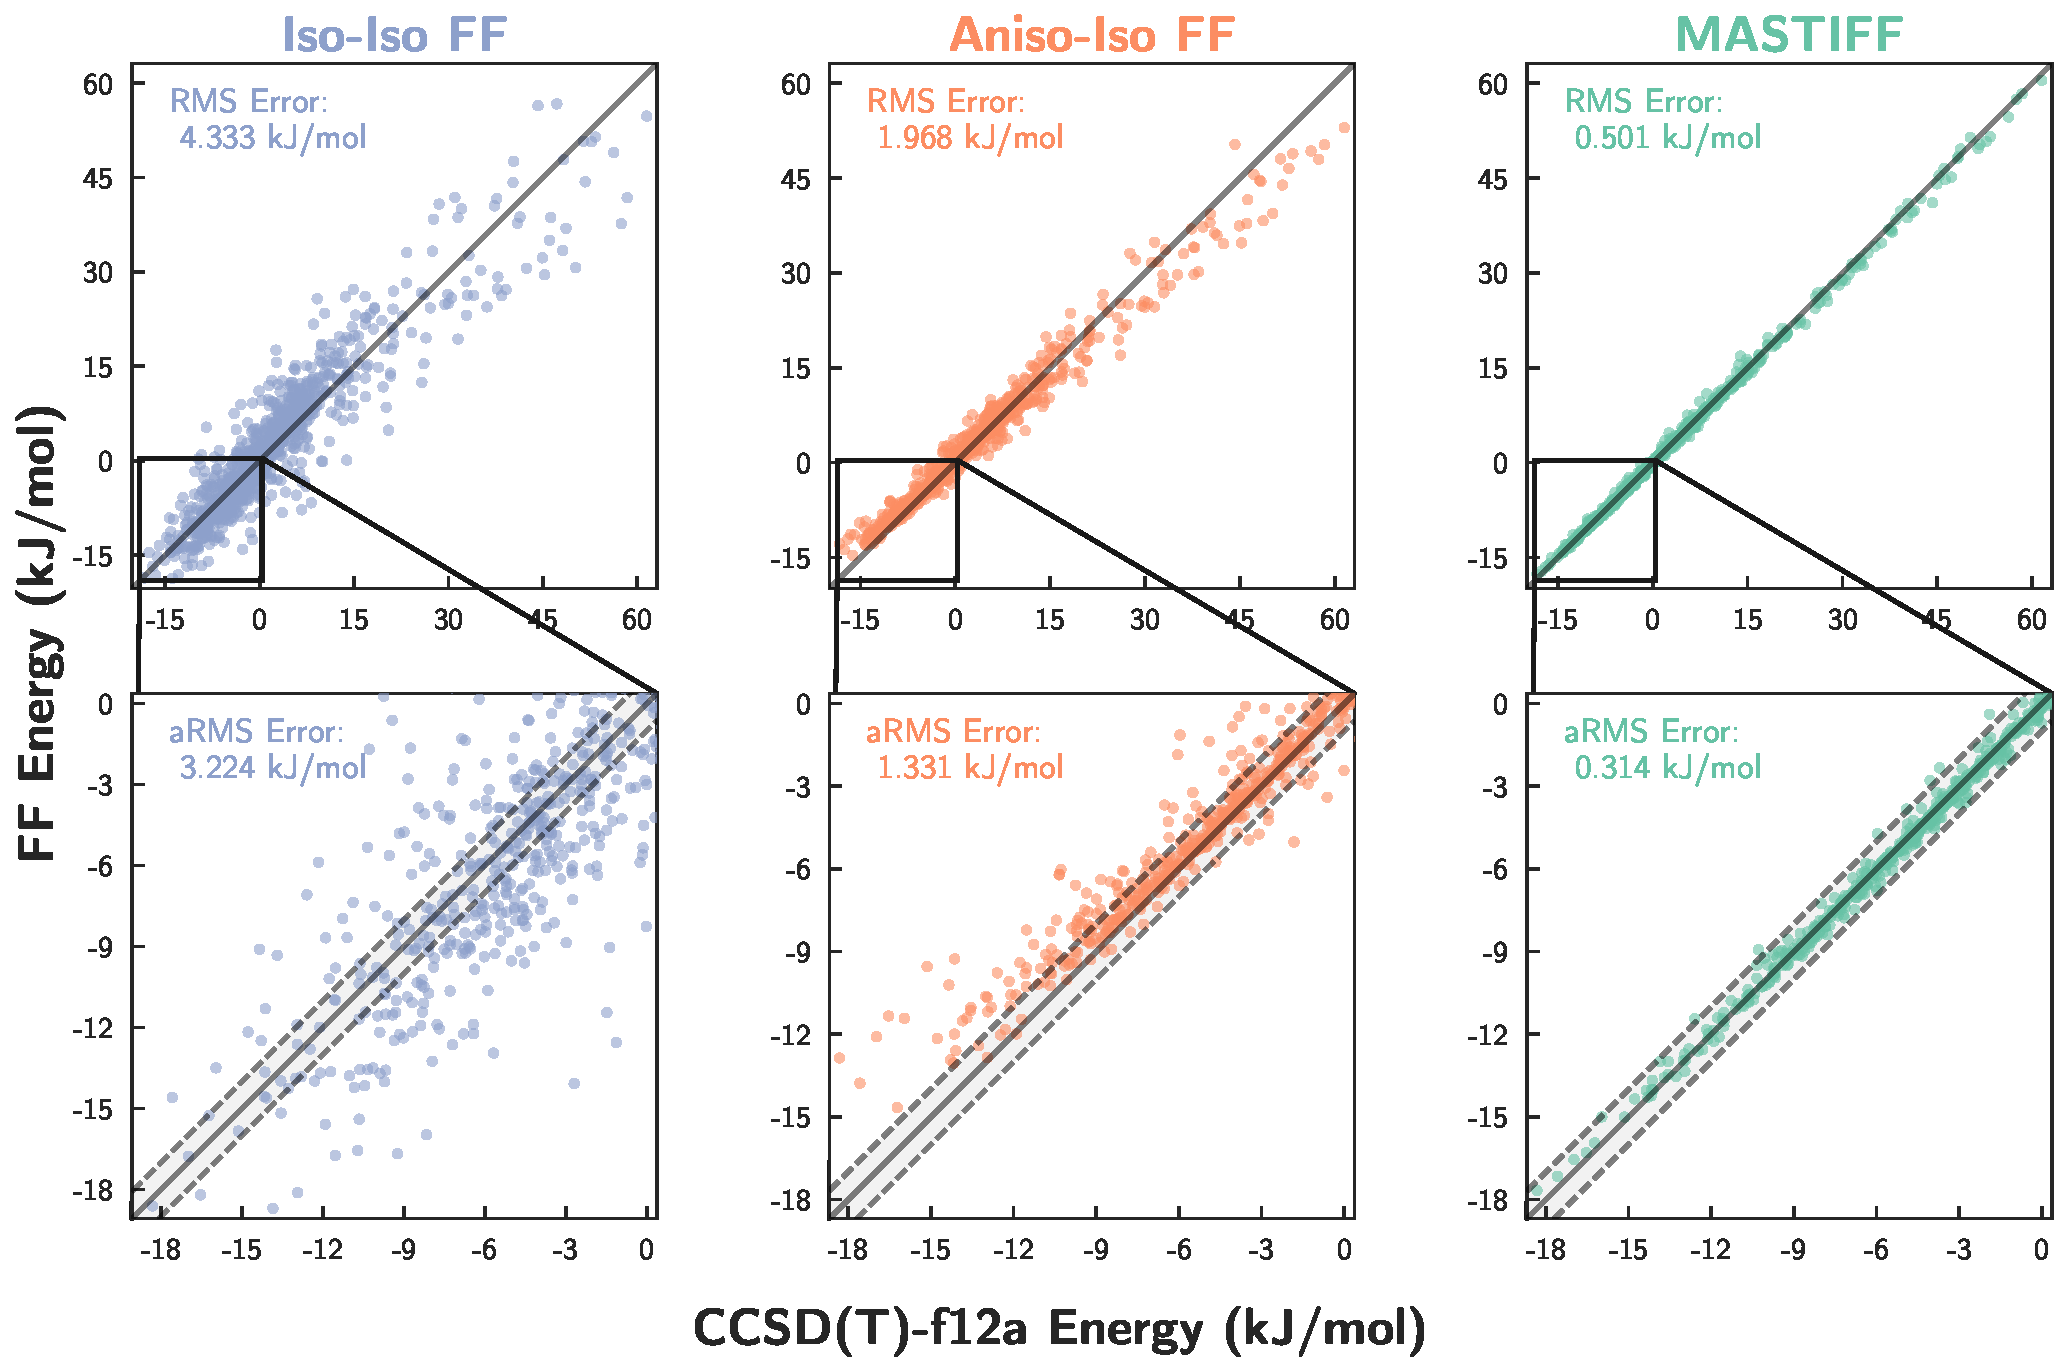
\includegraphics[width=0.9\textwidth]{anisotropic/scatterplots/h2o_h2o_comparison.pdf}
    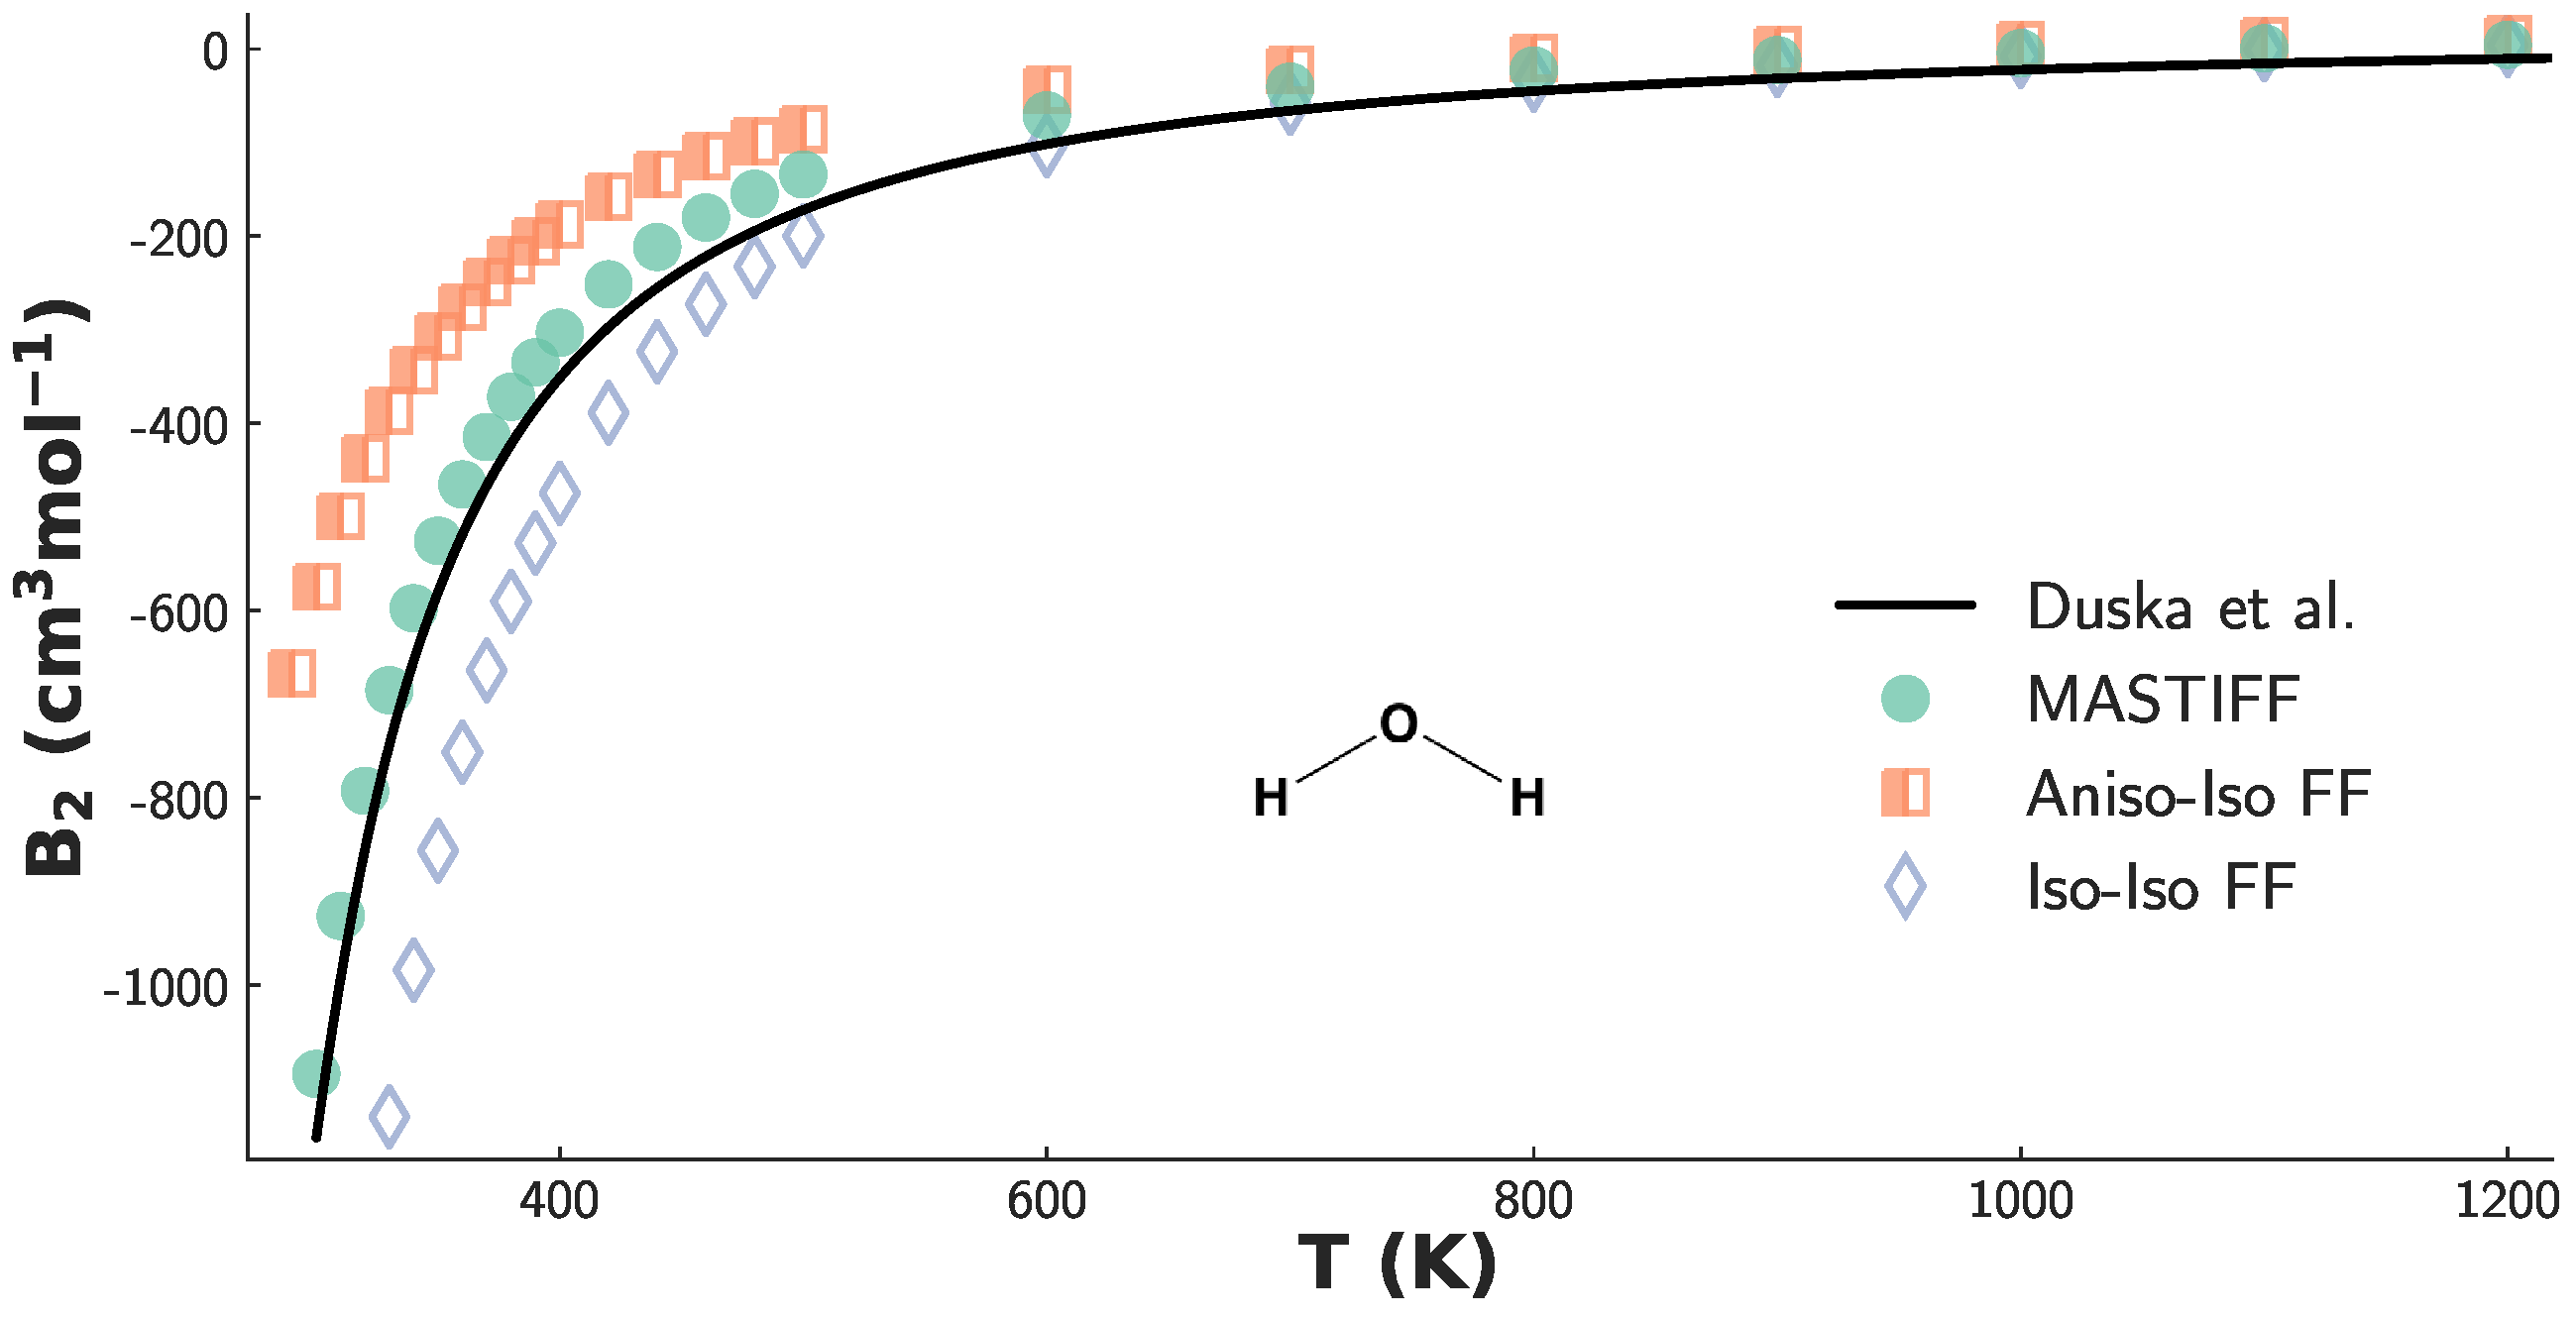
\includegraphics[width=0.9\textwidth]{anisotropic/virials/h2o/h2o_2nd_virial.pdf}
    \caption{
        Classical second virial for water. Experimental data from
            \citen{Duska2013}. 
        Note that some data points from \isoff extend below the plot area.
            }
    \label{fig:h2o_virial}
    \end{figure}
    %%%%%%%%%%%% H2O Comparison %%%%%%%%%%%%%
    %%%%%%%%%%%% H2O Comparison %%%%%%%%%%%%%
    \begin{figure}[ht]
    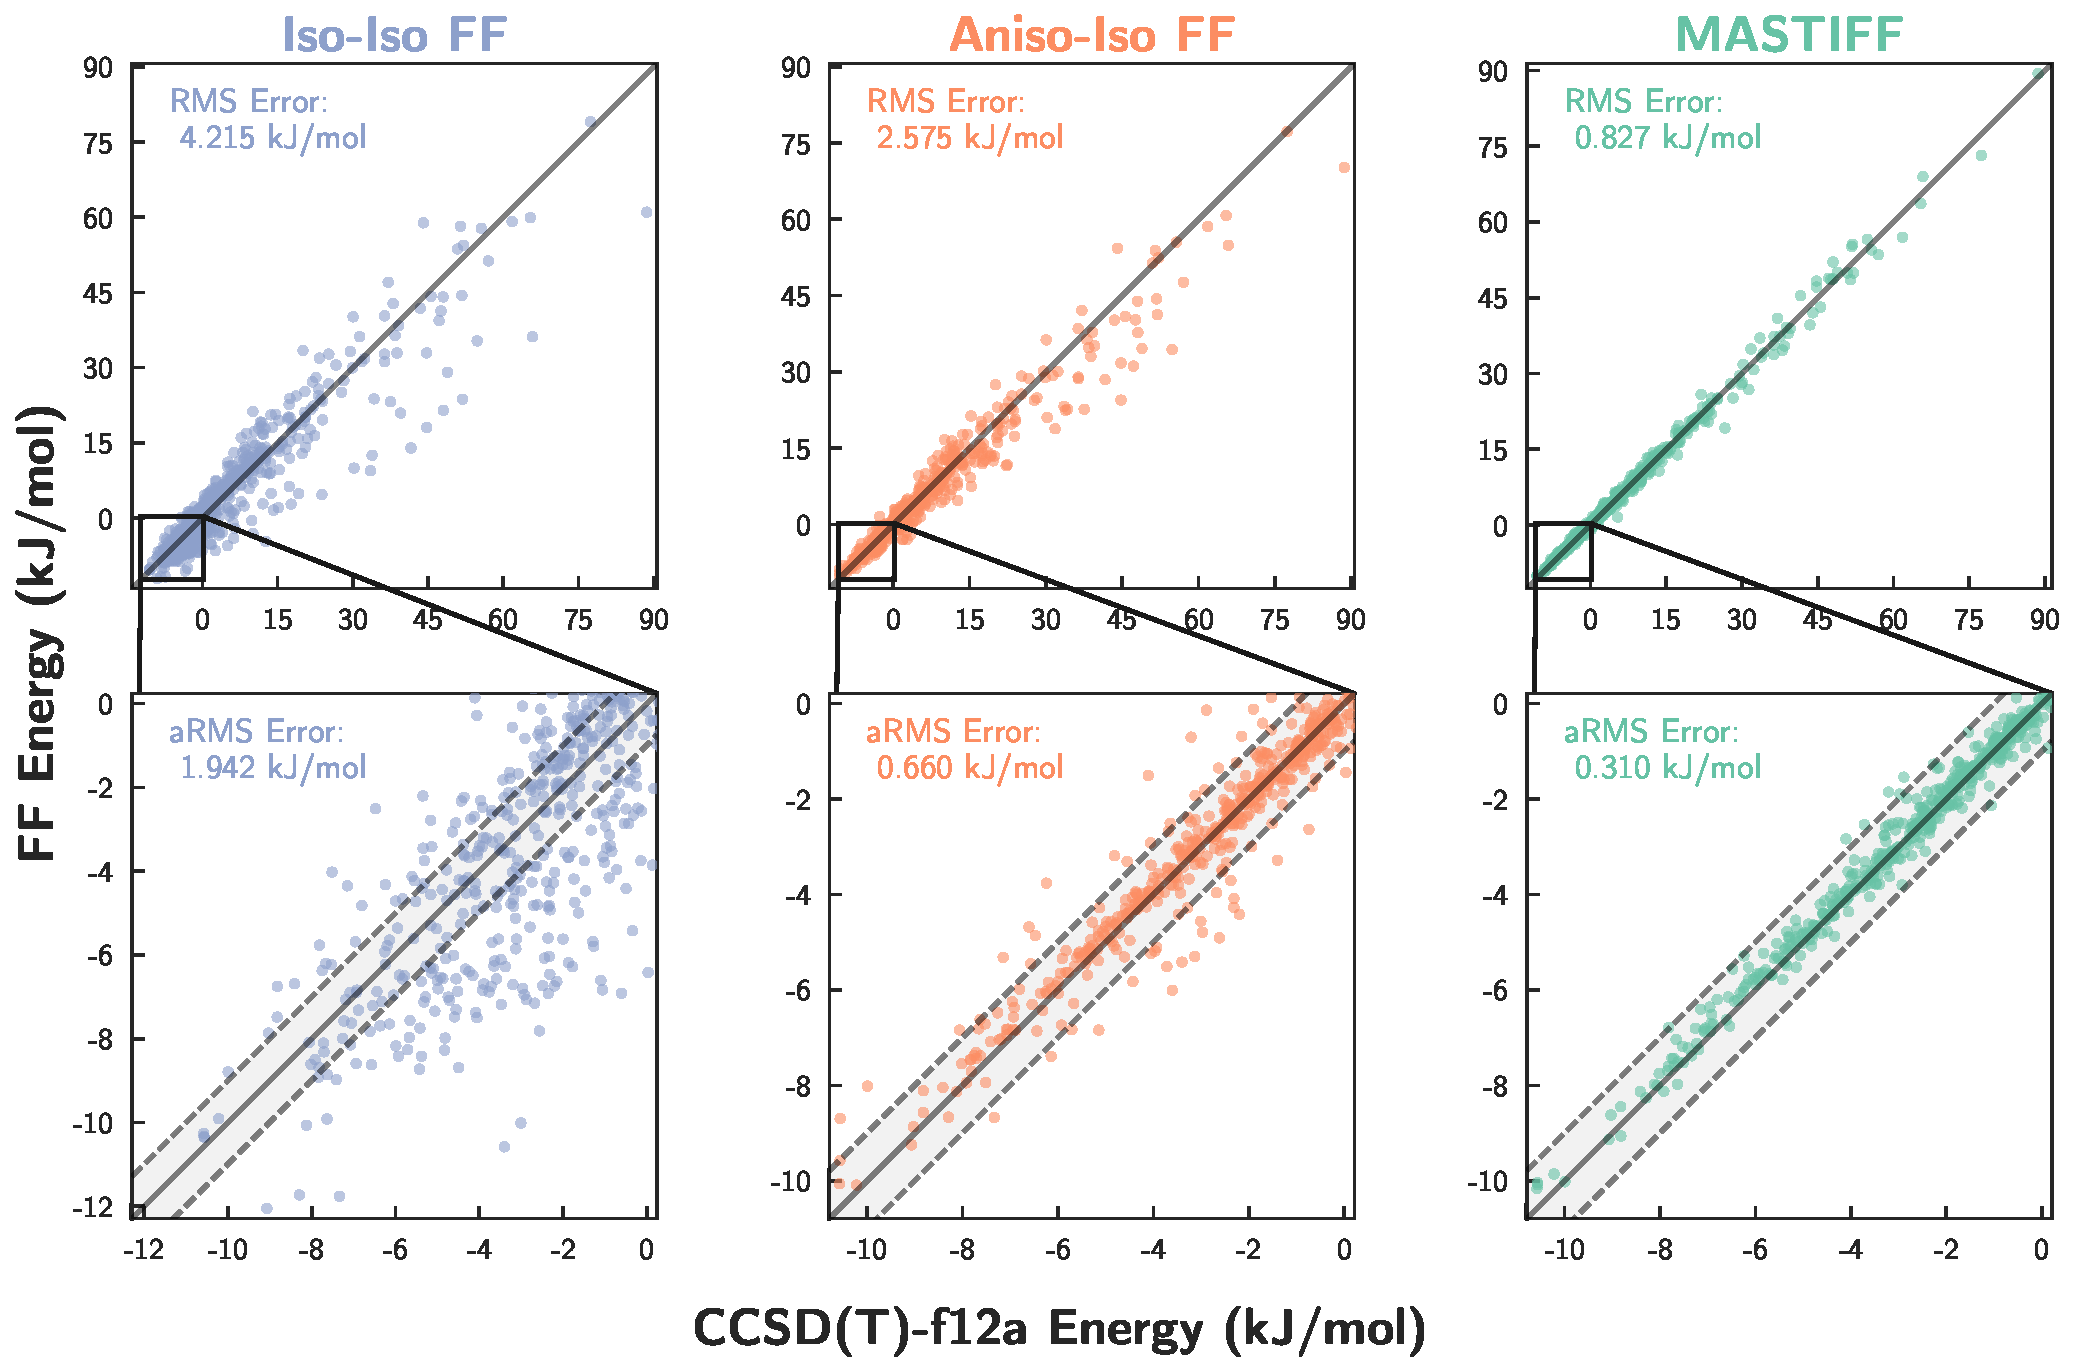
\includegraphics[width=0.9\textwidth]{anisotropic/scatterplots/nh3_nh3_comparison.pdf}
    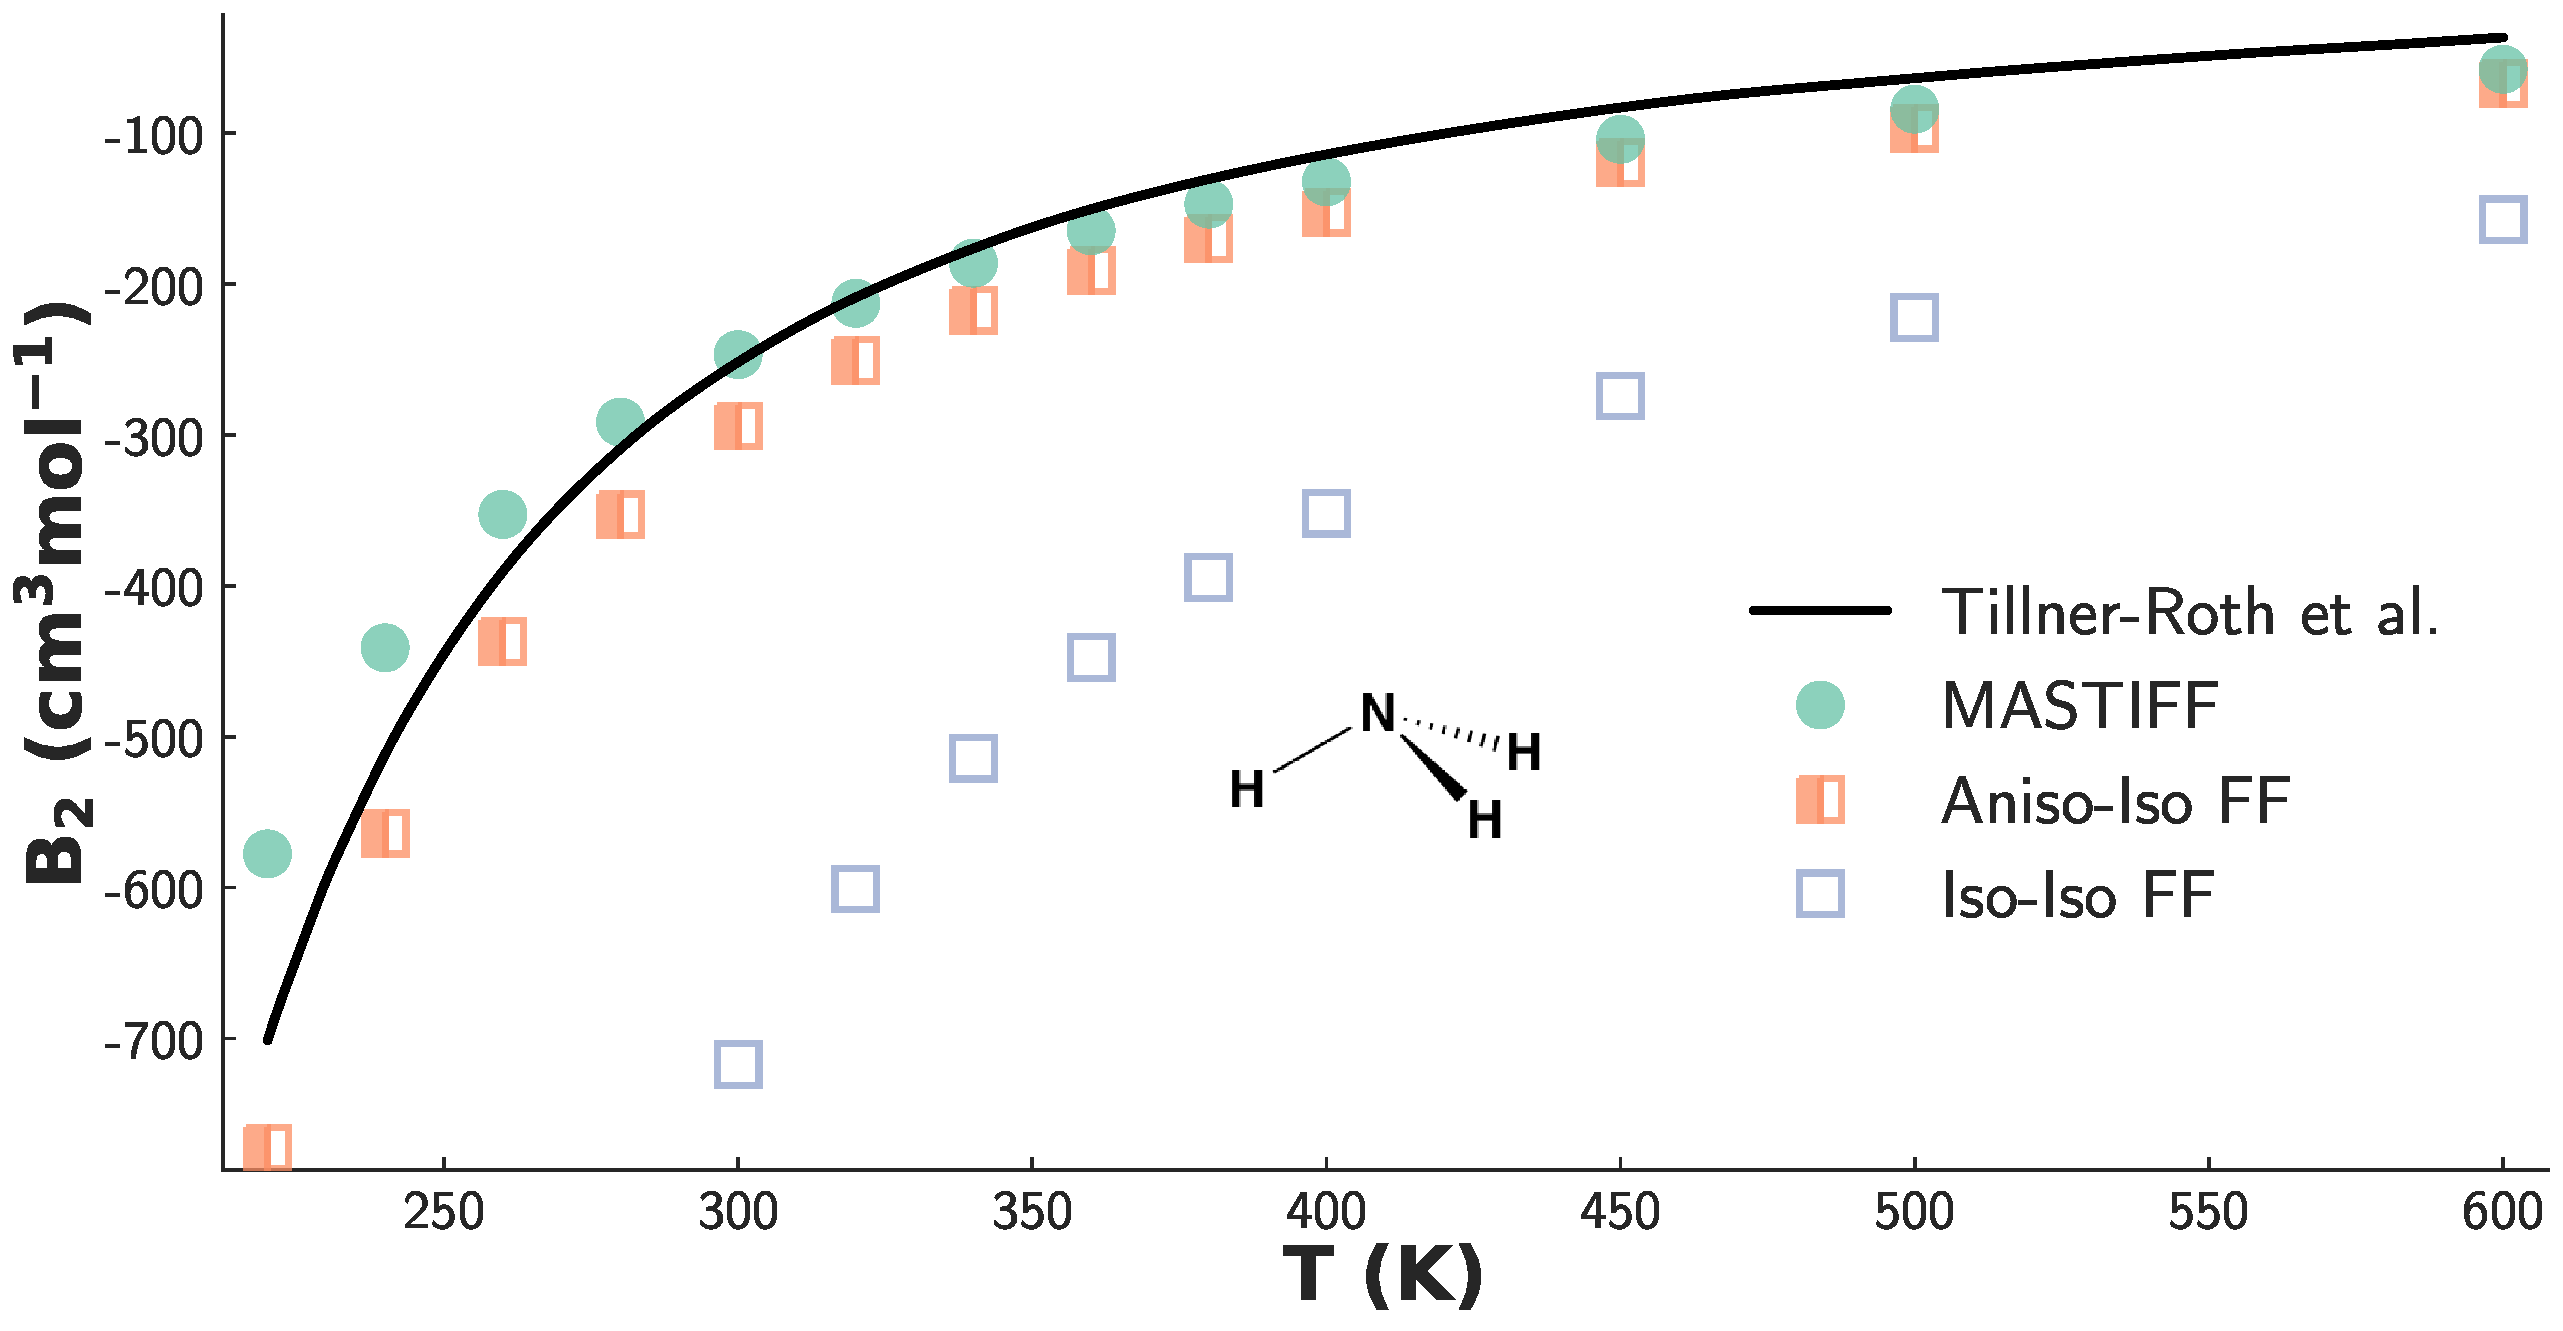
\includegraphics[width=0.9\textwidth]{anisotropic/virials/nh3/nh3_2nd_virial.pdf}
    \caption{
        Classical second virial for ammonia. Experimental data from
            \citen{tillner1993neue}.
        Note that some data points from \isoff extend below the plot area.
            }
    \label{fig:nh3_virial}
    \end{figure}
    %%%%%%%%%%%% H2O Comparison %%%%%%%%%%%%%
    %%%%%%%%%%%% H2O Comparison %%%%%%%%%%%%%
    \begin{figure}[ht]
    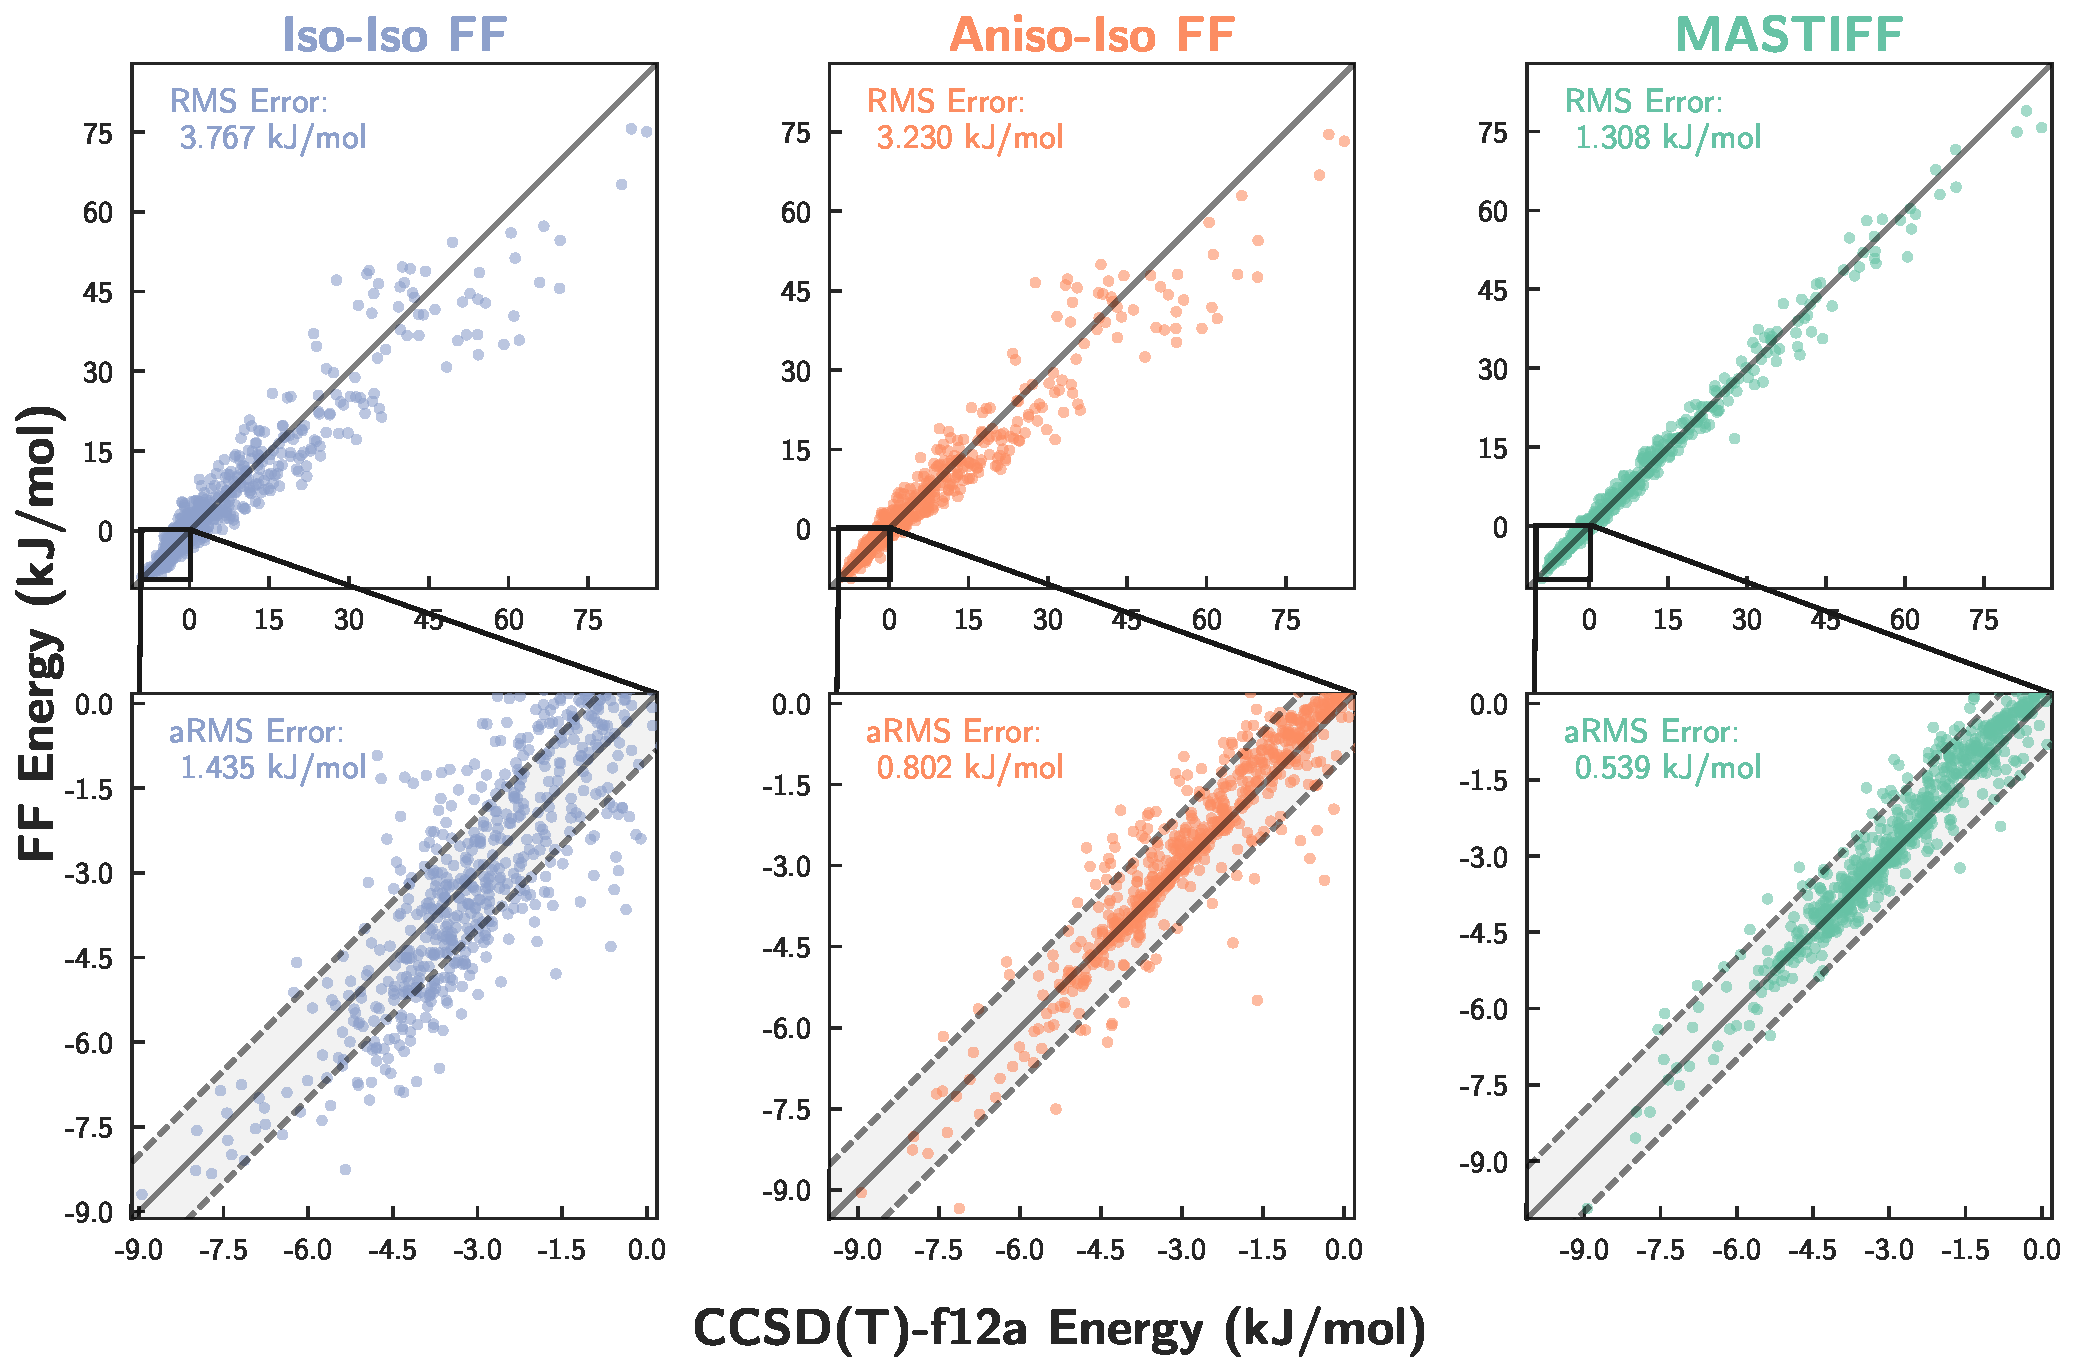
\includegraphics[width=0.9\textwidth]{anisotropic/scatterplots/chloromethane_chloromethane_comparison.pdf}
    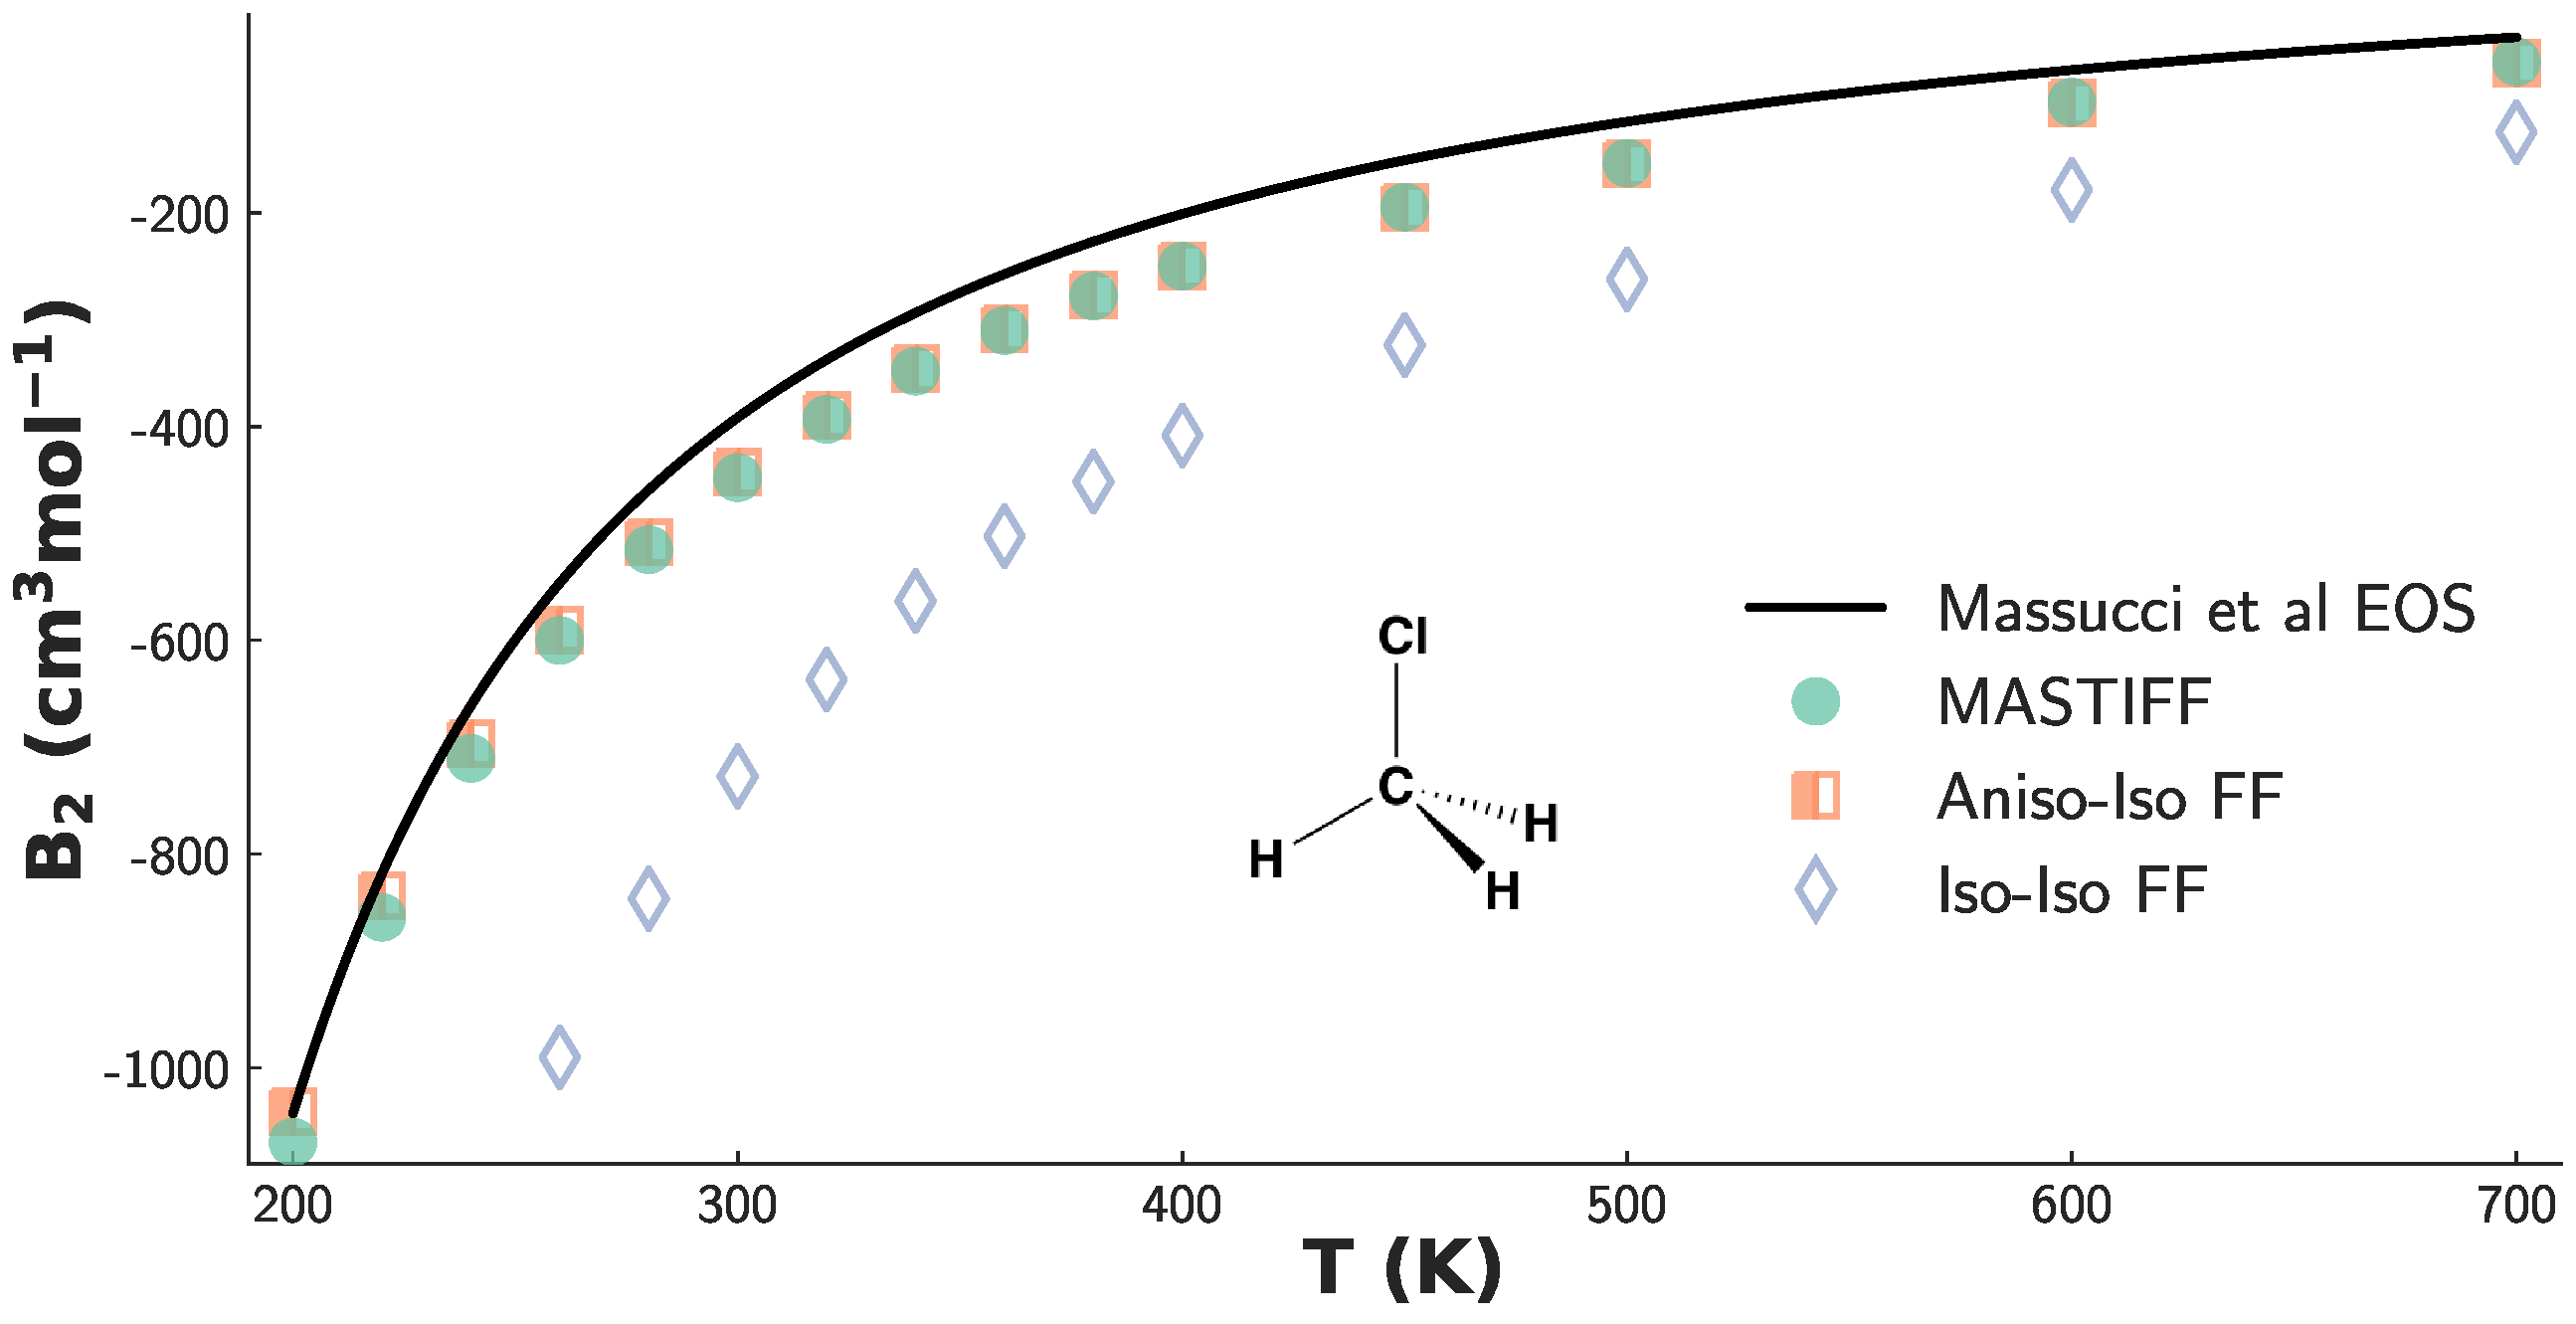
\includegraphics[width=0.9\textwidth]{anisotropic/virials/chloromethane/chloromethane_2nd_virial.pdf}
    \caption{
        Classical second virial for chloromethane. Experimental equation of
        state (EOS) from \citen{Massucci1998}.
        Note that some data points from \isoff extend below the plot area.
            }
    \label{fig:chloromethane_virial}
    \end{figure}
    %%%%%%%%%%%% H2O Comparison %%%%%%%%%%%%%
    %%%%%%%%%%%% Virial for CO2 %%%%%%%%%%%%%
    \begin{figure}[ht]
    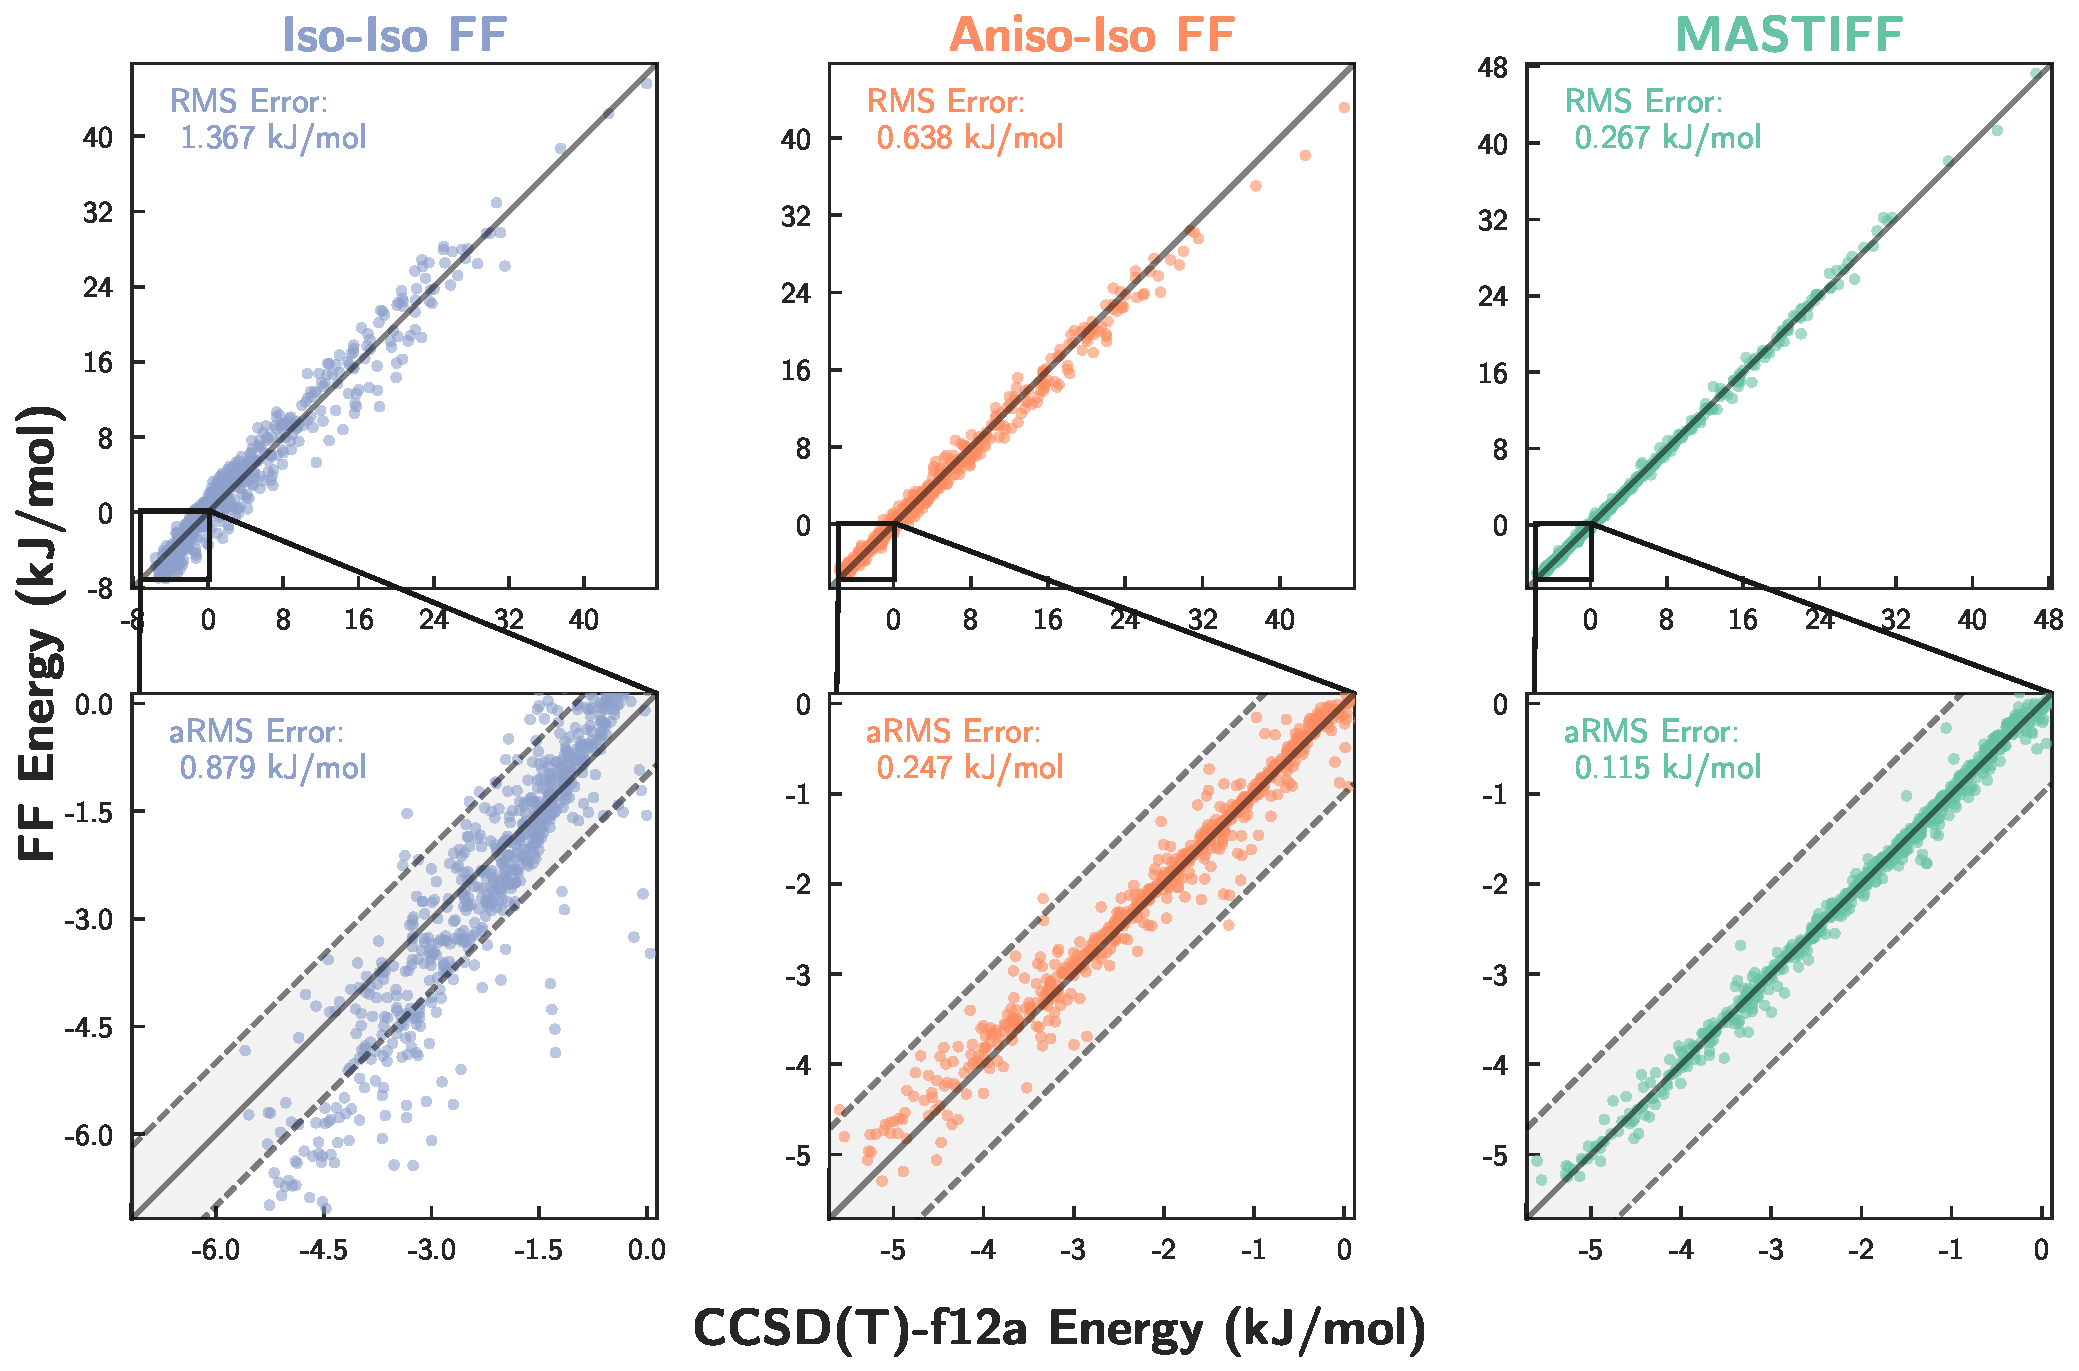
\includegraphics[width=0.9\textwidth]{anisotropic/scatterplots/co2_co2_comparison.pdf}
    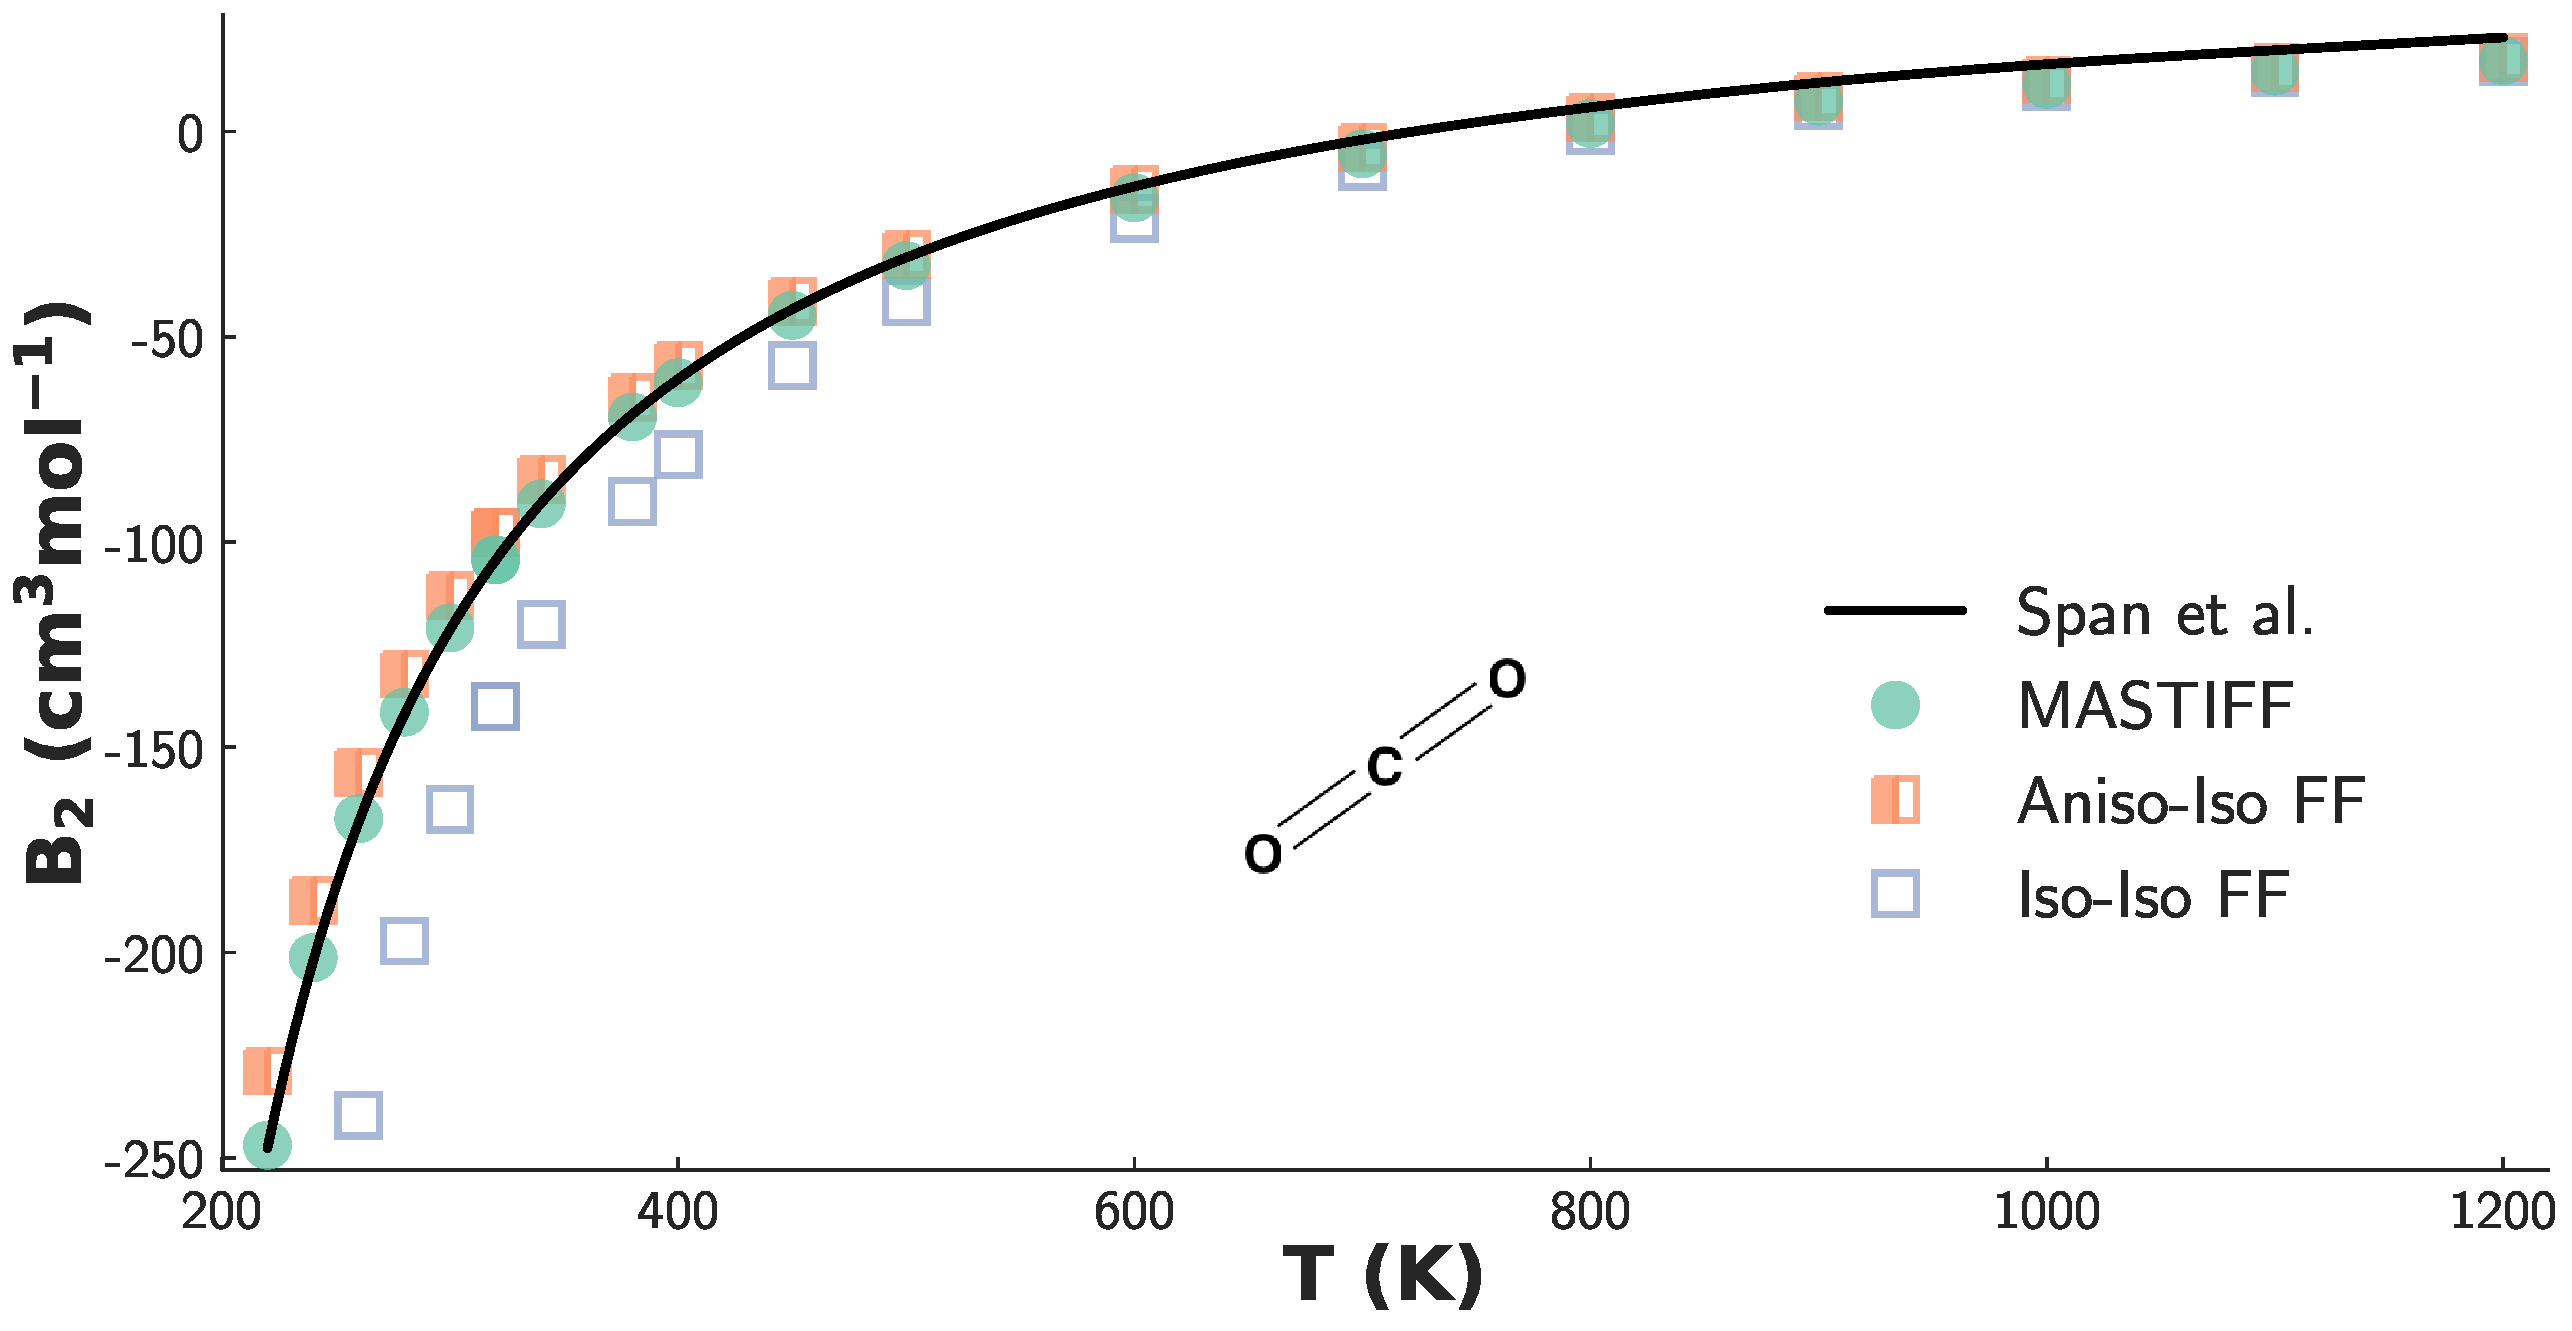
\includegraphics[width=0.9\textwidth]{anisotropic/virials/co2/co2_2nd_virial.pdf}
    \caption{
        Classical second virial for \co. 
        Experimental data from \citen{Span1996}
            }
    \label{fig:co2_virial}
    \end{figure}
    %%%%%%%%%%%% Virial for CO2 %%%%%%%%%%%%%
%
First,
we find that the \mastiff-CC
methodology predicts virial coefficients
which closely corresponds to experimental data. Given the range of systems
tested (\co dimer interactions are dispersion dominated, while \cl, \nh, and
\ho have relatively larger electrostatic and polarization contributions), 
this suggests that, when benchmarked against high-quality electronic structure
theory, our anisotropic methodology offers a general strategy for
quantitatively accurate
pairwise potential development. Second, we note that
the \isoff-CC 
predictions are much worse than their \mastiff-CC or \isaff counterparts, 
suggesting that
an accurate treatment of long-range electrostatics is essential to obtain
accurate virial coefficients.
Finally, though \isaff-CC gives equally good predictions for some systems
(notably \cl) compared to the \mastiff-CC method, 
virial coefficients for other systems (especially \ho) are less
accurate, suggesting that dispersion and short-range
anisotropies are also important in many systems for the accurate prediction of
virial coefficients. Consequently, and in summary, 
the minimal additional computational overhead (compared to \isaff-CC) and
excellent accuracy of \mastiff-CC permits us to recommend this fully anisotropic \mastiff methodology 
for the prediction of dimer interaction energies and second virial coefficients.


\clearpage
\end{subsection}
\begin{subsection}{Comparison to Experiment: Condensed Phase Properties of \co}
\label{sec:co2}

To demonstrate the applicability of the \mastiff methodology in condensed
phase simulation, we have developed a complete
many-body potential for \co, and have run bulk simulations involving a variety
of vapor, liquid, supercritical, and solid phase points for preliminary
comparisons to experiment.  As above, we use the \mastiff-CC
potential to describe the pairwise potential and the many-body induction.
As for other many-body effects, it
is well-known\cite{Yu2012b,Hellmann2017,Oakley2009a} that three-body
dispersion, and to a lesser extent, three-body exchange, are also
important.\cite{Desgranges2015} 
Thus, 
%% after testing a few combination-rule
%% compatible (so as to be easily
%% implemented in OpenMM) three-body potentials for their ability to reproduce the
%% \citeboth{Hellmann2017} three-body interaction energy database, 
we model three-body dispersion via a modified version of the three-body dispersion potential developed by
\citeauthor{Oakley2009a} (see \cref{sec:methods}).  Three-body exchange
effects are not accounted for in our model, however 
prior work shows they are very small under the conditions studied
here.\cite{Yu2012b}

Density predictions for the vapor, liquid, and supercritical phases of \co are
shown in \cref{tab:densities}, and enthalpies of
sublimation and vaporization are shown in \cref{tab:deltah}. 
%
We find it notable and highly encouraging that
\mastiff-CC reproduces \emph{all} studied experimental properties to within a
few percent. Of particular note is our excellent reproduction of the
sublimation enthalpy, which critically depends on the lattice energy of the
solid phase. Unlike with liquid or supercritical \co, where
many dimer configurations are sampled,
the
solid consists of only four symmetry-unique
configurations. Consequently, whereas an isotropic
potential (which is in error for particular dimer
configurations, but can take advantage of error cancellation to be accurate in an average sense) 
might yield good property predictions for the liquid phase, 
it would not be expected to correctly predict the solid phase (where beneficial
error cancellation is unlikely). 
Indeed, most theories (including our previously developed SYM-3B
model,\cite{Yu2012b} nearly all popular empirically-developed \co
models,\cite{Perez-Sanchez2013} AMOEBA,\cite{Heit2016a} and many electronic
structure theories\cite{Heit2016a}) struggle to correctly predict the solid phase
properties of \co! For this reason, 
the enthalpy of sublimation is
an extremely stringent test of force field
quality,\cite{Perez-Sanchez2013} 
and our accurate reproduction
of this quantity is evidence for both the excellent quality of the \mastiff-CC
potential in specific and of the importance of atomic-level anisotropy in
general.
Though more testing is needed to confirm
the accuracy of our anisotropic force field for
other phase points, our results suggest that, crucially, the
\mastiff-CC potential is transferable across the entire phase diagram of
molecular \co, and is capable of describing the gas, liquid, supercritical,
and solid phases. 

Despite the excellent success of the \mastiff-CC model, it is also worthwhile to
address and understand its minor shortcomings. In particular, we have studied 
representative two- and three-body energies taken from a snapshot of
the liquid at 273.15 K and 100 bar. For the two-body energies, we have compared
against the extremely accurate \citeboth{Kalugina2014} potential, while for
three-body energies we have benchmarked against the \citeboth{Hellmann2017}
PES. From these results (\cref{sec:mastiff-co2_snapshots}), 
it is clear that our pairwise
\mastiff potential is highly accurate for all configurations present in the
liquid, with very small \rmse and no systematic error in the
potential, such that the total two-body energy is accurate to within 0.05\%
compared to the \citeauthor{Kalugina2014} PES. Once again, this result argues
strongly for the accuracy and transferability of the \mastiff methodology, and
suggests that an inclusion of anisotropy is essential, not only for gas-phase
clusters, but also for simulations of the bulk. By contrast, our three-body
potential is systematically in error compared to the \citeauthor{Hellmann2017}
PES. Though some of this error may be due to inaccuracies in the
benchmark potential itself as compared to coupled-cluster,\cite{Hellmann2017}
most of this error is likely due to
inaccuracies in our model for many-body \co interactions. The
atomically-isotropic treatment of three-body dispersion, neglect of
higher-order dispersion terms ,
and neglect of explicit three-body exchange
may all contribute to this error, and
an improved model for many-body \co interactions will be the subject of future
research. Indeed, it is well-known that the density can be extremely sensitive
to the treatment of many-body effects,\cite{Desgranges2015} and it is highly
probable that an improved many-body model would reduce the already small
errors observed in our \mastiff-CC predictions.
Regardless, for now we conclude that, despite some small residual errors
arising from the simplified treatment of many-body effects, our \mastiff-CC
methodology yields for an extremely accurate force field for \co with
applicability across 
a range of experimentally-important phases.



%%%%%%%%%%%%%%%%%%%%% Macroscopic Properties %%%%%%%%%%%%%%%%%%%%%%%%%%%%%%%%%%
\begin{table}
%\small
\centering
\renewcommand\arraystretch{1.1}
\begin{tabular}{@{}lccccc@{}}
\hline
\toprule

Phase & T (K) & P (bar) &  Density (g/ml) &  Exp. & \% Error  \\

\midrule
Gas       & 300    &  50  & 0.131   & 0.128 &  2.34  \\
Supercritical & 320    & 140  & 0.728   & 0.703 &  3.56  \\
Liquid    & 300    & 100  & 0.825   & 0.802 &  2.87  \\
Liquid    & 273.15 & 100  & 1.000   & 0.974 &  2.67  \\
%
\bottomrule
\hline
\end{tabular}
\caption{
    Select densities for \co across a range of experimental conditions.
    Experimental data taken from the EOS of \citen{Span1996}.
    Entries ordered by increasing experimental density.
	}
\label{tab:densities}
\end{table}
%\normalsize
%%%%%%%%%%%%%%%%%%%%% Macroscopic Properties %%%%%%%%%%%%%%%%%%%%%%%%%%%%%%%%%%


%%%%%%%%%%%%%%%%%%%%% Macroscopic Properties %%%%%%%%%%%%%%%%%%%%%%%%%%%%%%%%%%
\begin{table}
%\small
\centering
\renewcommand\arraystretch{1.1}
\begin{tabular}{@{}lccccc@{}}
\hline
\toprule

Phases & T (K) & \deltah (\kjmolold) &  Exp. & \% Error  \\

\midrule
s $\to$ g   & 194.76 & $25.0 \pm 0.15$ &  25.2  &  -0.8  \\
l $\to$ g   & 288    & 7.92   &    7.80    &   -1.4 \\
%
\bottomrule
\hline
\end{tabular}
\caption{
    Enthalpies of vaporization/sublimation for \co at several temperatures. 
    Experimental data taken from the EOS of \citen{Span1996}.
    The uncertainty in the enthalpy of sublimation is due to ambiguity in the theoretical zero-point energy for \co (see
    \cref{sec:methods}. 
	}
\label{tab:deltah}
\end{table}
%\normalsize
%%%%%%%%%%%%%%%%%%%%% Macroscopic Properties %%%%%%%%%%%%%%%%%%%%%%%%%%%%%%%%%%



\end{subsection}



%% Explain MSE Fits
%%     Exchange:
%%     Electrostatics:
%%     Dispersion: 
%%     Total Energy:

